% !TEX program = xelatex
\documentclass{matthijs}

\newcolumntype{R}{>{\arraybackslash}m{10cm}}

% First/last page style and page ornaments
\usepackage{wallpaper}
\usepackage{color}
\definecolor{arobsblue2}{HTML}{0e2642}
%\definecolor{arobsblue}{HTML}{0f2c4c}
\definecolor{arobsblue}{HTML}{0e335c}
\definecolor{invisible}{rgb}{1,1,1}
%\ULCornerWallPaper{1}{asset_bg_top.jpg}
%\LRCornerWallPaper{1}{asset_ornament.png}
%\LLCornerWallPaper{1}{asset_ornament_3f.png}

% Confirm geometry (already set in cls)
% This is needed for fancyhdr
\geometry{a4paper} %paper format
\geometry{margin=2.75cm} %margins

% Page numbering
\usepackage{fancyhdr}
\usepackage{lastpage}
\pagestyle{fancy}
\fancyhf{}
\fancyhead{}
\renewcommand{\headrulewidth}{0pt}
\lfoot{\textcolor{invisible}{\gitAbbrevHash~\gitAuthorName~\gitAuthorIsoDate}}
\rfoot{\textbf{\thepage}\hspace{1ex}of\hspace{1ex}\pageref{LastPage}}

% Bibliography
\usepackage{csquotes}
\usepackage[style=ieee]{biblatex}
\addbibresource{research.bib}
\renewcommand*{\mkbibacro}[1]{#1}
\setcounter{biburllcpenalty}{7000}
\setcounter{biburlucpenalty}{8000}

% Versioning
\usepackage[maxdepth=2]{gitinfo2}

% This lets the text look really juicy
\usepackage[verbose=errors,babel=true]{microtype}
\usepackage{extdash}

% Figures
\usepackage{amsmath}
\usepackage{tikz}
\usepackage{pgfplots}
\usepgfplotslibrary{polar}
\pgfplotsset{compat=1.18}
%\usetikzlibrary{fadings}
%\tikzfading[
%	name=arobsfade,
%	inner color=transparent!0,
%	outer color=transparent!100
%]

%\usepackage{atbegshi}
%\AtBeginShipout{
%	\begin{tikzpicture}[remember picture,overlay]
%		\fill (current page.north west) node[below right,fill=arobsblue2,draw=arobsblue2,minimum width=\paperwidth,minimum height=2ex] (box) {};
%		\clip (current page.north west) node[below right,draw=none,minimum width=\paperwidth,minimum height=2ex] (box) {};
 %      	%\clip (current page.north west) node[minimum width=\paperwidth, minimum height=2ex, preaction={fill=arobsblue2, draw=arobsblue2}] (box) {};
%		\clip[preaction={fill=red,draw=red}] (current page.south east) rectangle (5cm, 5cm);
%		\clip (current page.south west) rectangle (current page.north east);
%
%		\fill (current page.north west) [below right, overlay, green, path fading=arobsfade, draw=none] circle (20cm);
%	\end{tikzpicture}
%}

\usepackage{environ}
\NewEnviron{largequation}{
	\begin{equation*}
		\scalebox{1.2}{
			$\BODY$
		}
	\end{equation*}
}

\begin{document}

	% Set language to English
	\taal{en}

	% Turn off page numbering
	\pagenumbering{gobble}

	% Cover page
	\begin{titelpagina}
		\color{white}

		\titel{\vspace{50pt}Research into Lane Detection Algorithms for FPGAs}{\emph{Project Lane Detection using FPGAs}}
		\author{
			\begin{tabular}{r l}
				\textbf{Author:} & Matthijs Bakker{\color{white}\footnote{\color{white}\textsuperscript{1} s1142121@student.windesheim.nl}} \\
				\textbf{Course:} & HBO-ICT ESA Full-Time \\
				\\
				\textbf{Company:} & AROBS Transilvania SA, Cluj-Napoca, Romania \\
				\textbf{Company Supervisor:} & Pangyu Jeong \\
				\textbf{Windesheim Supervisor:} & Willie Conen \\
				\\
				\textbf{Version:} & 0.1 \\
				\textbf{Commit:} & \gitAbbrevHash @master \\
			\end{tabular}
			\vspace{8ex}
		}

		\ThisULCornerWallPaper{1.001}{asset_bg_first_page.jpg}
		
	\end{titelpagina}

	\begin{hoofdstuk*}{Abstract}

		\thispagestyle{empty}

		\textbf{[todo:]}

	\end{hoofdstuk*}

	\begin{inhoudspagina}

	\end{inhoudspagina}

	\pagenumbering{arabic}

	\lefthyphenmin=3
	\righthyphenmin=3
	
	\begin{hoofdstuk}{Introduction}

		A run-off-road crash is a type of accident involving a single vehicle in which it veers off the road and collides with a natural or artificial object \cite{liu2009factors}.
		A study conducted in 2008 by the U.S. Department of Transportation indicated that 45 percent of all fatal highway crashes in the USA that year were run-off-road crashes \cite{dod2011run}.
		For more than 95 percent of these run-off-road crashes, the cause of the crash was attributed to the driver of the vehicle \cite{dod2011run}.
		Another report published by the University of Minnesota shows that the aforementioned number may be as high as 53 percent \cite{edwards2013pilot}.
		In that report, numerous countermeasures were proposed to alert the driver if their car was headed off the road, such as delivering haptic feedback through the steering wheel and giving auditory warnings to the driver.
		However, while countermeasures were proposed, this paper did not clarify when these countermeasures should be triggered or how the car should detect if it is veering off the road.
		
		\bigskip

		To improve the safety of vehicles, AROBS has been developing an Advanced Driver\Hyphdash Assistance System -- hereafter referred to as an ADAS.
		This system comprises of numerous subsystems which monitor and control certain processes inside of the car.
		One of these subsystems is the Lane Departure Warning System \cite{el2020novel}.
		As the name implies, this component of the ADAS assists the driver in keeping the vehicle within in a road lane.
		To detect if the car is properly centered, a camera is positioned on the dashboard of the car and it is faced towards the road.
		The approximate position of the vehicle relative to the road lane is calculated by feeding the video feed from the camera through an algorithm.
		If the result of this process indicates that the car is deterring from the lane, a signal is sent to the ADAS so that a warning can be provided to the driver of the vehicle.
		
		\bigskip

		The goal of this research is to select the best suited algorithm for detecting \textbf{road lane markings} from a video feed and calculating the approximate location of the car relative to the lane.
		It is vital that we spend time on making sure that the selected algorithm fits with the project, because the next phase of the project depends on the information that is gained from this research.

		\bigskip

		This paper is written using the IMRaD format, because it is what we were taught to use at Windesheim.
		However, I realised that this might not be the best format to write the paper in, because the literature study section was exceptionally big compared to the other sections.
		As advised by my mentor, I moved the literature study to a separate section before the main part of the paper.
		I tried to spread out the findings in this section as much as possible by creating (sub-)paragraphs for different topics.

	\end{hoofdstuk}
	
	\begin{hoofdstuk}{Literature Study}

		First of all, I will set up a literature study to search for existing lane marking algorithms by using various online document aggregators such as Google Scholar and ResearchGate.
		It will be interesting to gauge which algorithms are used in similar projects, because it helps us narrow down on the wide choice of available algorithms.
		Because some papers share common stages in their algorithm, like the usage of the Sobel operator or the Hough transform, I will gather more information on these stages and why they are used in this field.
		It will also be helpful to search if people have made optimizations or variations upon these standard procedures.
		An example of such a variation is an optimized straight-lane Hough Transform targeting FPGAs \cite{el2020novel} which has a higher performance ceiling because it can be parallelized.
		By taking into account existing optimizations and previous work from other research, we can speed up the process and increase the quality of the product.

		\bigskip

		The methods used in the papers that were analyzed shared a common theme: first, the input video feed would be preprocessed and cleaned from artifacts, before being ran through a feature extraction technique like the Hough Transform, and finally being subjected to a line classification technique.
		This preprocessing stage is of high importance, because it directly affects the effectiveness of the feature extraction phase.
		If the features of the image are not properly highlighted, the level of detail remains too high and the feature extraction technique might pick up photographic artifacts as lines \cite{felix2003low}.

		\begin{paragraaf}{Image Preprocessing Techniques}

			According to Malmir et al. \cite{malmir2019design} the main source of difficulty for lane detection is the variation of operating conditions in captured road images.
			An example of this is the variation in colors of the paint used for drawing road markings.
			White paint is common in Europe while yellow paint can be seen in North America.
			The yellow gloom of the sunset can make it harder to detect yellow lane markings on a video frame because they blend in with the environment \cite{tumasov2021research}.
			Though, the use of white paint has a disadvantage as well: pools of water can reflect sunlight and appear as white lane markings \cite{krine2021road}.
			To generify our product and make it work in many different environments, we need to take into account such environmental factors.
			The video feed needs to be preprocessed in such a way that as little artifacts as possible get fed into the Hough transform.
			This decreases the chance that anomalies appear in the result of the Hough transform.
			
			\begin{subparagraaf}{Grayscale Conversion}

				A grayscale image is one in which the only colors are shades of gray \cite{fisher2003hypermedia}.
				The benefit of converting an image to grayscale is that the contrast between the black/gray part of the road and the bright white/yellow road markings increases \cite{tanksale2019finding}.
				The contrast within the image significantly increases which makes the feature extraction phase more effective \cite{ebrahimpour2012vanishing}.

				\bigskip

				Formally, the intensity value of a pixel in a grayscale image is called the \textit{luminance} \cite{itu2017recommendation}.
				The luminance ranges from black at the weakest intensity to white at the strongest \cite{johnson2006stephen}.
				I chose to pick the values recommended by the BT.601-7 standard \cite{itu2017recommendation} because these have also been used in the \textit{rgb2gray} function in the MATLAB standard library.
				The formula that will be applied to each pixel pixel is mentioned in \verwijzingb{figuur}{Formula for calculating the luminance of a pixel}.
				In this formula, $E_Y$ is the luminance of the pixel and $E_{R,G,B}$ are the values of the color channels.

				\begin{figuur}{Formula for calculating the luminance of a pixel}
					\begin{equation*}
						E_Y = 0.299 E_R + 0.587 E_G + 0.114 E_B
					\end{equation*}\cite{itu2017recommendation}
				\end{figuur}
			
			\end{subparagraaf}

			\begin{subparagraaf}{Region of Interest Definition}

				To reduce the computing resources needed to run the algorithm, regions of interest (ROIs) may be defined around where the left and right lane markings are supposed to be \cite{el2020novel}.
				The pixels outside of the defined ROIs will not be processed by the algorithm.
								
				\bigskip

				The location of the ROI depends on the installation position, height and viewing angle of the camera and has to be calibrated once per installation \cite{malmir2019design}.
				It can be assumed that the upper portion of a video frame captured by the dashboard camera is above the horizon, meaning that it is not worth scanning for road lanes.
				Thus, it can be safely ignored to save computing resources.
				An example of this scenario can be seen in \verwijzingb{figuur}{Example use case of a Region of Interest}, where \textit{(a)} is the input image and \textit{(b)} is the defined ROI.

				\begin{figuur}{Example use case of a Region of Interest}
					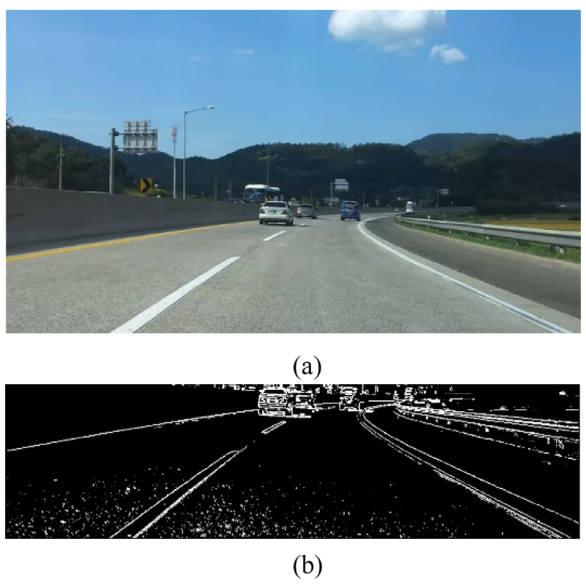
\includegraphics[width=0.5\textwidth]{malmir2019design-img1.png}
					\cite{malmir2019design}
				\end{figuur}

			\end{subparagraaf}

			\begin{subparagraaf}{Noise Reduction}

				It is inevitable that images from a camera will contain some amount of noise.
				To prevent that noise is mistaken for edges in the edge filtering phase of our algorithm, the image must be cleaned up before it is delivered to the edge detector \cite{sarab2020canny}.

				\begin{subsubparagraaf}{Pixel Average Filter}

					A pixel average filter operates by computing an average or arithmetic mean of the grayscale intensity values for each pixel position in a set of captured images from the same scene \cite{spring2001image}.
					Neighbor pixels don't affect the value of a target pixel, which makes this technique highly suited to be implemented in parallel.
					
					\begin{figuur}{Equation for a pixel average filter on a sequence of video frames}

						\begin{equation*}
							A (N, x, y) = \frac{1}{N} \cdot \sum_{i=1}^{N} I (i, x, y)
						\end{equation*}\cite{spring2001image}
					
					\end{figuur}

					The equation in \verwijzingb{figuur}{Equation for a pixel average filter on a sequence of video frames} can be used to determine the intensity value $I$ of the pixel at the coordinate $(x,y)$ in frame $i$ out of $N$ total frames.
					A downside of this algorithm in the form of the aforementioned equation is that it needs historic data; applying it on a single frame won't have any effect on the output of that frame.
					This historic data also needs to be kept available in order for future frames to be calculated, requiring computer memory.
					It is also possible to use a variant of the algorithm which uses a rolling average instead of historic data \cite{spring2001image} as seen in \verwijzingb{figuur}{Equation for a rolling average variant of a pixel averaging filter}.

					\begin{figuur}{Equation for a rolling average variant of a pixel averaging filter}

						\begin{equation*}
							A (N, x, y) = \frac{I (x, y) + (N - 1) \cdot A (N - 1, x, y)}{N}
						\end{equation*}\cite{spring2001image}
					
					\end{figuur}

					The equation looks complex, but the storage of the rolling average value can be easily implemented in VHDL using an intermediate variable or signal.
					Accessing the little amount of memory that a FPGA has is time intensive, making memory operations expensive.
					Therefore, the method as described in \verwijzingb{figuur}{Equation for a rolling average variant of a pixel averaging filter} is more suitable for implementation on FPGAs.
				
				\end{subsubparagraaf}

				\begin{subsubparagraaf}{Gaussian Filter}

					In order to reduce the noise in the Hough Transform accumulator, a blur is applied to the image beforehand.
					The blur reduces detail and eliminates noise in the source image \cite{fan2016faster}.
					The advantage of using Gaussian Blur is that edges in the image get treated similarly no matter their direction \cite{waltz1998efficient}.
					Another advantage is that this algorithm uses filter kernels which can be convoluted with the source image in parallel \cite{stroem2016parallel}.
					
					\begin{figuur}{Formula for generating a two-dimensional Gaussian kernel}

						\begin{largequation}
							K(x,y) = e^{-(\frac{(x - x_o)^2}{2 \sigma x^2} + \frac{(x - y_o)^2}{2 \sigma y^2})}
						\end{largequation}\cite{gedraite2011investigation}
					
					\end{figuur}

					\bigskip

					In \verwijzingb{figuur}{Formula for generating a two-dimensional Gaussian kernel} the $ (x_0,y_0) $ is the origin and $x$ and $y$ are the distances from the origin in Cartesian space \cite{gedraite2011investigation}.
					Symbol $\sigma$ represents the standard deviation of the Gaussian distribution, which affects how much the neighbor points are weighed; thus affecting the strength of \mbox{the blur \cite{haddad1991class}.}
					The output of the function, $K(x,y)$, is the resulting kernel which we can convolute with an image.
					This kernel is a matrix which is used to determine which weights need to be applied to the neighbors of a specific pixel in the image; each pixel's new value is a weighted average of that pixel's neighborhood \cite{gedraite2011investigation}.
					Convoluting it with an image has a similar effect to a low-pass filter, smoothing the lines of the image \cite{haddad1991class}\cite{ferreira2010imagej}.

					\bigskip

					The goal is to pick a blur strength that will reduce noise enough so that no false edges get picked up by the Hough Transform, but that the lane marking lines will be kept intact.
					\mbox{Fan et al. \cite{fan2016faster} recommended} a kernel size of $ K_x = K_y = 3 $ and a strength of $ \sigma = 1.5 $ for this purpose.
					A visual representation of this kernel with approximate values is shown in \verwijzingb{figuur}{Example of a Gaussian kernel}.
					
					\begin{figuur}{Example of a Gaussian kernel}

						\vspace{-2ex}% this thing is big! uwu

						\begin{equation*}
							\begin{bmatrix}
								0.094742 & 0.118318 & 0.094742 \\
								0.118318 & 0.147761 & 0.118318 \\
								0.094742 & 0.118318 & 0.094742 
							\end{bmatrix}
						\end{equation*}

						$K_x = K_y = 3$ \\
						$\sigma = 1.5$
					
					\end{figuur}
					
					\bigskip

					The convolution of the Gaussian kernel with the image can be described as in the formula in \verwijzingb{figuur}{Formula for two-dimensional image convolution}, where $K$ is the kernel matrix and $x,y$ are the kernel indices.
					The input image is represented as $a$, the output image as $b$, and the indices of these images as the parameters $i$ and $j$.
					
					\begin{figuur}{Formula for two-dimensional image convolution}

						\begin{equation*}
							b(i, j) = \sum_{x = -\infty}^{\infty} \sum_{y = -\infty}^{\infty} K(x, y) \cdot a(i - x, j - y)
						\end{equation*}
						\cite{sneha2018convolution} (modified symbols to fit with text)
					
					\end{figuur}

					\bigskip

					To determine the value of a pixel, the Gaussian kernel must have information on the neighboring pixels.
					Because the pixels at the edge of the image don't have neighboring pixels (assuming the kernel size is larger than one) they get cut off.
					Is is also visible in the formula in \verwijzingb{figuur}{Formula for two-dimensional image convolution} that the pixels get cut off (see $x(i-x, j-y)$).
					This explains why the resolution of the output image is smaller than that of the input image.
					\verwijzingb{figuur}{Formulae for calculating the dimensions of the result image} suggests how to calculate the width and height of the resulting image based on the resolution of the initial image and the size of the Gaussian kernel.
					In these formulae, $w$ is the width of an image and $h$ is the height of an image.
					Symbols $x$ and $y$ represent the width and height of the Gaussian kernel.

					\begin{figuur}{Formulae for calculating the dimensions of the result image}
						\begin{equation*}
							w_{out} = w_{in} - 2 * (\lfloor\frac{x - 1}{2}\rfloor + 1)
						\end{equation*}

						\vspace{-4ex}
					
						\begin{equation*}
							h_{out} = h_{in} - 2 * (\lfloor\frac{y - 1}{2}\rfloor + 1)
						\end{equation*}
					\end{figuur}

					\bigskip

					In scenarios where the aforementioned pixel cutoff is undesirable, a technique known as \textit{zero padding} can be applied.
					\mbox{According to Sneha \cite{sneha2018convolution}, zero} padding is done when there are no image pixels to overlap the kernel pixels, like at the borders of an image.
					At the place of each non-overlapping pixel of the kernel matrix, a zero-valued image pixel gets inserted.
					When convolution is done, a zero-padded value will remain to be zero because the resulting product of the multiplication of all the color channels is also zero.
					The benefit of this technique is that the addition of zeroes to the image does not alter the image in any sense except for its size \cite{sneha2018convolution}.

				\end{subsubparagraaf}

			\end{subparagraaf}

			\begin{subparagraaf}{Edge Detection}

				\textbf{[todo:]}

				\begin{subsubparagraaf}{Sobel-Feldman Operator}

					Sampling window

					\textbf{[todo:]}

				\end{subsubparagraaf}

				\begin{subsubparagraaf}{Canny Edge Detector}

					This edge detection technique is not an operator in itself; it suggests a routine around an existing edge detection operator such as the Sobel-Feldman operator.
					\textbf{[todo:]}

				\end{subsubparagraaf}

			\end{subparagraaf}

			\begin{subparagraaf}{Thresholding}

				\textbf{[todo:]}

			\end{subparagraaf}

		\end{paragraaf}

		\begin{paragraaf}{Feature Extraction Techniques}

			\textbf{[todo:]}

			\begin{subparagraaf}{Hough Transform}

				The Hough Transform is a technique which can be used to isolate features of a particular shape within an image \cite{fisher2003hypermedia}.
				The classical variant is of this technique is mostly used to detect basic predefined shapes such as lines and ellipses.
				Derivations of this variant such as the Generalized Hough Transform can be employed in applications where a simple analytic description of a feature is not possible \cite{fisher2003hypermedia}.
				The advantage of the Hough transform is that pixels lying in one line need not all be contiguous.\cite{kahl2000hough}
				This is useful when trying to detect road markings because these lines often have breaks in them.

				\begin{figuur}{Equation of a line using Hesse normal form}
					\begin{equation*}
						\rho = x \cdot cos \theta + y \cdot sin \theta
					\end{equation*}\cite{caltech2009line}
				\end{figuur}

				Lines can be uniquely represented by using the distance from the line to the origin and the angle of the line.
				These parameters are represented by $\rho$ and $\theta$ respectively \cite{caltech2009line}.
				The idea behind the Hough Transform is that we map the Cartesian space of the image (represented by $x,y$) to the parameter space of lines \cite{solberg2009hough}.
				For each pixel in the Cartesian space, we can represent all the possible lines through it by a single line in the parameter \mbox{space (see \verwijzingb{figuur}{Transformation of a single point to a line in the Hough space}).}
				This means that all pixels which lie on the same line in the Cartesian space are represented by lines which all pass through a single point in the parameter space \cite{kahl2000hough}.

				\begin{figuur}{Transformation of a single point to a line in the Hough space}
					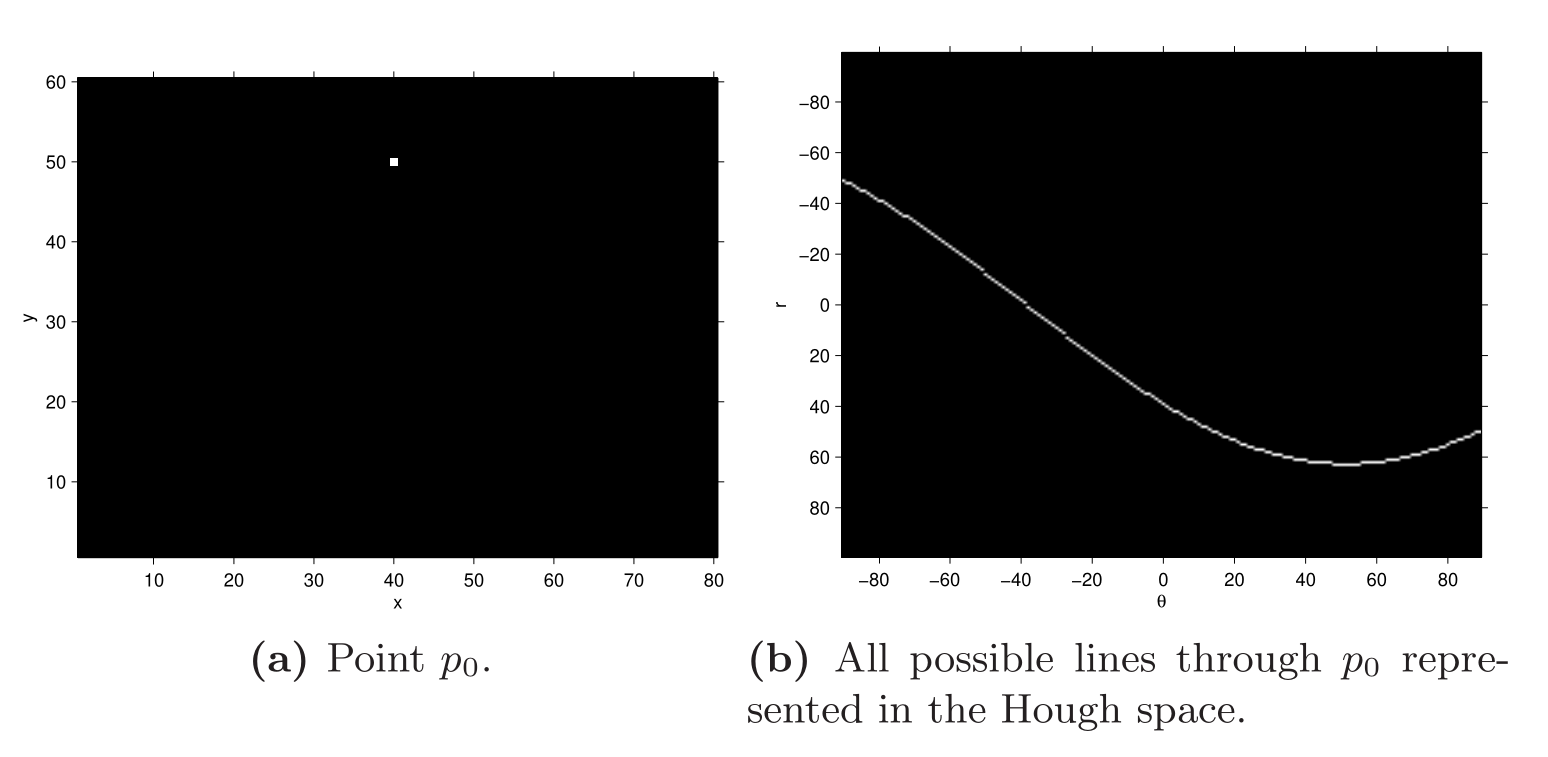
\includegraphics[width=0.9\textwidth]{caltech2009line-img1.png}
					\cite{caltech2009line}
				\end{figuur}

				\bigskip

				First, the parameter space gets quantized into a two-dimensional matrix $ A[\rho,\theta] $ which is initialized with zeroes \cite{solberg2009hough}.
				This matrix is often referred to as the accumulator or the Hough space.
				Then, we loop over the image in Cartesian space and increment each element of the accumulator which corresponds to an edge point determined by our preprocessing stage.
				The accumulator can be visualized as a histogram which shows the frequency of the edge points corresponding to values in the parameter space (i.e. those that lie on a common line) \cite{kahl2000hough}.
				The peaks of this histogram correspond to lines in the \mbox{Cartesian space (see \verwijzingb{figuur}{Examples of the accumulator spaces of Hough transforms}).}
				Finally, we can determine the position $\rho,\theta$ of the lines by thresholding the values from the histogram so that we only keep the peaks.

				\begin{figuur}{Examples of the accumulator spaces of Hough transforms}
					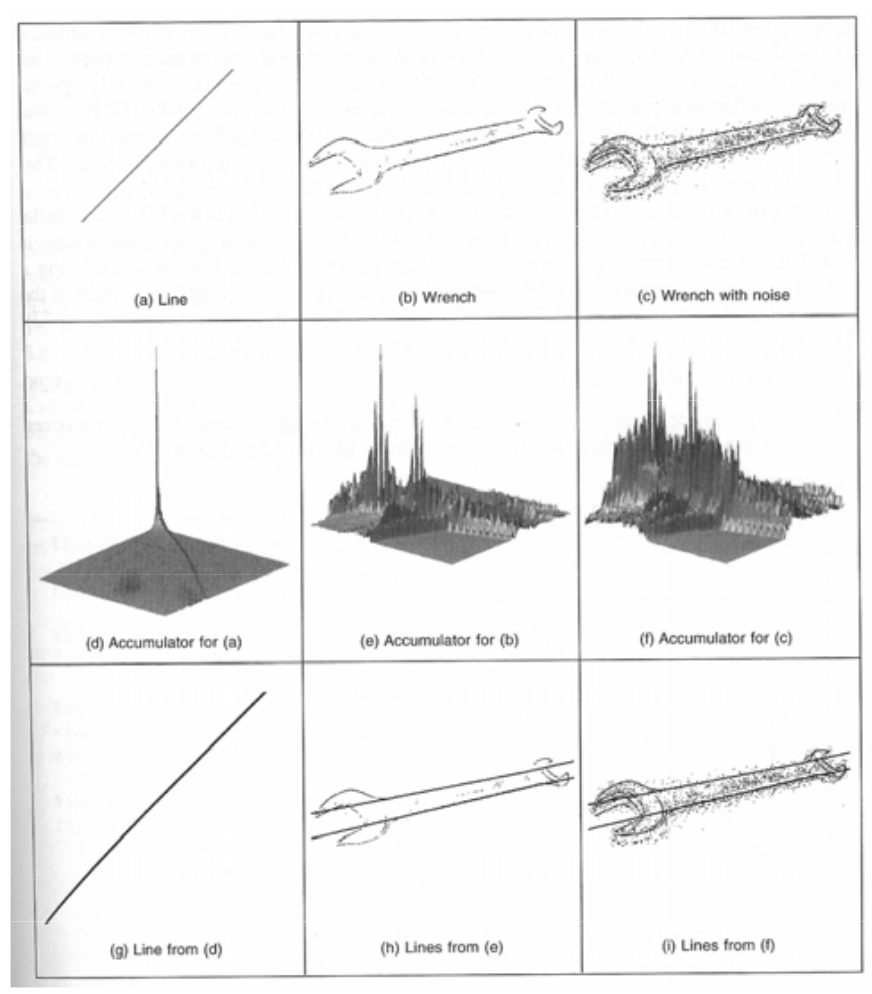
\includegraphics[width=0.5\textwidth]{solberg2009hough-img1.png}
					\cite{solberg2009hough}
				\end{figuur}

				The polar coordinates of the resulting lines can be converted to Cartesian coordinates using the formulae in \verwijzingb{figuur}{Formulae for converting polar coordinates of a line to Cartesian coordinates} where $p$ can be the first or second point of the line.
				
				\begin{figuur}{Formulae for converting polar coordinates of a line to Cartesian coordinates}
					\begin{equation*}
						x_p = \frac{(\rho - y_p sin \theta)}{cos \theta}
					\end{equation*}

					\vspace{-2ex}

					\begin{equation*}
						y_p = \frac{(\rho - x_p cos \theta)}{sin \theta}
					\end{equation*}

					\vspace{1ex}

					\cite{dawkins2018polar}
				\end{figuur}
			
				\begin{subsubparagraaf}{Time and Space Complexity}
					Although the Hough transform is widely used, its high time and space complexity are serious downsides that are challenging to manage when implementing it on embedded systems \cite{dongkyun2008real}.
					Assuming the size of a video frame is 1280 by 720 pixels and 10 percent of these pixels are edge points, the total number of multiplications are $1280 \cdot 720 \cdot 0.1\theta \cdot 2 $ and the total number of additions is $1280 \cdot 720 \cdot 0.1\theta$ \cite{dongkyun2008real}.
					The space complexity is related to the memory needed to store the parameter space, which is influenced by the image resolution, $\rho$ and $\theta$.
					Assuming the size of a video frame is 1280 by 720 pixels, the size of one accumulator cell is $\lceil (log_e(1280)/log_e(2)) \rceil$ bits and the size of the accumulator is $\rho \cdot \theta$.
					Theoretically, we need at least 2 bytes of memory to fit each accumulator cell, meaning that we need a total of $16 \cdot(900 \cdot 2) \cdot 180$ bytes to store the parameter space for a 1280 by 720 video frame.
					The main bottleneck of the Hough Transform comes from the amount of chained read and write memory operations; some cell values in the parameter space are read and increased by one, so the next calculated value must wait until this accumulating operation is finished \cite{dongkyun2008real}.
					
					\bigskip

					The Arty A7 35T -- our target FPGA development board -- only has 1800 kibibits \cite{digilent2020arty} of fast Block RAM, meaning that we cannot fit the entire accumulator in it.
					We have to decide if we want to use the slower DDR3L RAM of which we have plenty, or decrease the needed space for the accumulator by using other prescribed techniques such as downscaling or ROI definition.
					According to the Arty A7 reference manual \cite{digilent2020arty}, the Artix FPGA chip includes $90$ DSP slices of type 48E1.
					These can be used to implement fully parallel digital signal processing algorithms like FIR filters, Fast Fourier transforms and NN pattern detection \cite{xilinx2018series}.
					Zhou et al. \cite{zhou2013efficient} used a combination of $178$ DSP48E1 slices and $3240$ kibibits of BRAM to create a parallel Hough implementation which can process a 512 by 512 image with 33232 edge points in $\approx 135.75 \mu s$.
					This was done on a very expensive Virtex FPGA which had plenty of DSP slices and BRAM available, and thus not realistic to implement as a product.
					Chuquimia et al \cite{chuquimia2018fpga} proposed a real time Hough Transform architecture on an Artix-7 FPGA using $2800$ kibibytes of BRAM and $153$ DSP48E1 slices for processing a 1920 by 1080 image in $\approx 32 ms$
					In addition to my assigned FPGA development board only having ninety DSP slices, I have no prior experience with them and there doesn't seem to be much documentation about them from Digilent.
					Therefore, I am not too keen on using this technology.

				\end{subsubparagraaf}

				\begin{subsubparagraaf}{Vanishing Point-Based Optimizations}

					Road lane markings are typically at an angle between 45 and 90 degrees when viewed from a dashboard camera.
					Knowing this, we can adapt the Hough Transform to only compute between these angles.
					There exist multiple ways to do this:

					\begin{itemize}

						\item Specify subdivisions in the $\rho\theta$ plane such that the peaks outside these areas are not taken into account in the thresholding phase \cite{solberg2009hough}
						\item Restrict the accumulation stage to only increase the accumulator values that correspond to $ max > \theta > min $ \cite{looges1993hough}
					\end{itemize}

					However, we can further decrease the angle by looking at the vanishing point position in the road scene \cite{shang2011lane}.

				\end{subsubparagraaf}

			\end{subparagraaf}

			\begin{subparagraaf}{Radon Transform}

				\textbf{[todo:]}

			\end{subparagraaf}
		\end{paragraaf}

		\begin{paragraaf}{Line Classification Techniques}

			The resulting data from the Hough transform does not bear any meaning on its own \cite{gupta2016automated}.
			It consists of a set of lines that can represent anything; from actual road markings to anomalies in the roadside or cracks in the road.
			The goal of the classification part of the algorithm is to detect which lines are the left and right lane markings.

			\begin{subparagraaf}{Clustering of HT Results}

				The Hough Transform used in the feature extraction phase gives us the extremes of the lane marking lines \cite{gupta2016automated}.
				To convert these extremes into usable data, it must be clustered and grouped into line segments.
				Clustering is grouping of unlabeled data points in such a way that the data points within the same group are similar to each other and the data points in different groups are dissimilar to each other \cite{sharma2020kmeans}.
				From the size and spread of the resulting clusters, we will be able to determine if a cluster represents a road lane marking.
				\bigskip

				$k$-means clustering allows us to find groups of similar entries within a dataset such that the total variance within groups is minimised \cite{martin2019implementing}.
				For grouping lines, a two dimensional variant of the Lloyd algorithm is used because each pixel of the line has a $x$ and $y$ value.
				A special attribute of the Lloyd algorithm is that the accuracy of clustering is increased at every iteration.
				Ebrahimpour et al. \cite{ebrahimpour2012vanishing} proposed to use this algorithm on the start and end points of each probabilistic Hough line to find the averages of these lines and to find the vanishing point of the image.
				They found that four iterations of Lloyd's algorithm are enough to reliably determine the averages of the lines.
				Dias et al. \cite{dias2020parallel} designed a FPGA architecture for Lloyd's algorithm that can run an iteration on 4096 two-dimensional data points within $8500 \mu s$.
				It required around 50 percent of the registers and around 80 percent of the LUTs available on their Kintex-7 FPGA, making it too exhaustive to run on an Artix-7.

				\bigskip

				Tumasov et al. \cite{tumasov2021research} proposed to use the DBSCAN algorithm to cluster the lines from the Hough Transform.
				This algorithm is highly suitable for situations in which different groups have a small difference in density.
				Line segments belonging to a lane have densities which are uniform or nearly uniform \cite{niu2016robust}.
				The difference between DBSCAN and $k$-means clustering is that the latter is a partitioned algorithm, which means that the final goal of the algorithm is to find the nearest densest neightbours instead of the transitive closure computation \cite{shi2014fpga}.
				What this means in our situation is that outliers like roadside artifacts will get ignored in DBSCAN clustering and only the high density areas such as the lines will get clustered.
				If we were to use $k$-means clustering, all of the input data would get considered when forming a result, including the outliers.
				Shi et al. \cite{shi2014fpga} implemented parallel DBSCAN which can be horizontally scaled over a FPGA.

			\end{subparagraaf}

			\begin{subparagraaf}{Stripe Detection}

				According to Malmir et al. \cite{malmir2019design}, the Hough transform stage achieves acceptable results 80 percent of the time.
				They suggested that this number decreases during non-ideal conditions such as poor visibility and driving at night time.
				In their work, they proposed a processing stage that occurs after an iteration of the Hough transform and provides reference data for the next iteration.

				\bigskip

				The basic premise of stripe detection is that the difference between video frames is not substantial because they are captured at a high rate.
				Therefore, we may use the stored coordinates of the detected lines in the previous frame as a reference while processing the current frame \cite{malmir2019design}.
				If the difference between the position of the lines in the previous frame and the current frame is within a predefined threshold, we can assume that are the same.
				Else, we distribute candidate points -- so-called 'particles' -- around the position of the line from the previous frame.
				Each particle has a rectangular search area around it.
				In this search area, a convolutional directional edge detection filter is applied to magnify the image features.
				Two kernels are used to find the left- and right edges of the lane marking.
				Once these edges are found, an additional test makes sure that the average brightness of the pixels between the edges on the grayscale image is brighter than that of the surrounding pixels.
				The position of the lane marking is found by stringing together the valid particles.

				\bigskip

				As mentioned in their paper, the effectiveness of this algorithm is highly dependent on the integrity of the result of the Hough transform that is carried out on the first frame of the video feed.
				This is because the algorithm bases its conception of correctness on previous frames of the video.
				The authors tried to overcome this issue by processing the video feed with a stricter threshold until a valid lane marking is found \cite{malmir2019design}.

			\end{subparagraaf}

		\end{paragraaf}

	\end{hoofdstuk}
	
	\begin{hoofdstuk}{Methods}

		\begin{paragraaf}{Test Implementation}

			A trend I have noticed among research on computer vision topics is that researchers first implement the proposed algorithms in MATLAB or a Python script before creating the end product.
			This approach to researching sounds good to me because it gives me a chance to prove that I am not only able to write about these algorithms but that I'm also able to put them to use.
			I'm not yet familiar with the previously mentioned programming languages, so I will use the C language instead.
			F\'elix et al. \cite{felix2003low} concluded from their research that modeling algorithms in ANSI C before modeling them in VHDL helped to reduce the time needed for the hardware implementation.
			This justifies the time that will be spent on the computer program.

			I will implement the algorithms that are most widely used among the mentioned research papers.
			These will be implemented in a computer program which will be able to run test images through them to determine how effective they are.
			The final chosen algorithm pipeline will be implemented on a Field Programmable Gate Array (FPGA), because it needs to be a low-cost device that can analyze the video feed in real-time.
%			A selection process will occur, in which the candidate algorithms will be judged by the following metrics:

			This final pipeline will be judged on the following factors:

			\begin{enumerate}

				\item	Accuracy of detection; the effectiveness of the pipeline on test images.
					This metric will be measured by implementing the pipeline into a computer program which can process test images.
					The pipeline will be ranked by how accurate the end result is compared to the reference result.

				\item	Environmental suitability; how well the pipeline works when put in different environments.
					This criterium involves using test images that were captured in different weather conditions, lighting conditions and different areas of the world.
					Particular detection techniques might work better than others in bright lighting, but may not work at all when the vehicle is driving through a tunnel or at night time.
					The selected test images, as seen in \verwijzingb{tabel}{List of test images}, were captured under many different circumstances.
					This metric is measured by the least amount of test images failed to process.

				\item	The feasibility of implementing the pipeline in digital logic.
					It is hard to set up concrete criterium for measuring this metric, because the time and knowledge required to implement particular algorithms depends on many factors, and it can't be properly calculated in advance.
					For this reason, I will estimate the difficulty of implementing the pipeline in hardware and I will assign it a score between one and five, with five meaning it would be very difficult to implement.

				\item	The resources required to run such an pipeline in real-time.
					We want as little delay as possible between the video frame being shot and the completion of the calculation.
					The quicker the car can detect that it's veering off the lane, the quicker the situation can be rectified, and the safer the system becomes.
					After all, the safety of human lives are at stake.\\
					This metric will be measured by:

					\begin{itemize}

						\item	The average amount of milliseconds it takes for a reference implementation to process one frame
						
						\item	The amount of Look-Up Tables, Flip-Flops and Block RAM a reference implementation occupies

					\end{itemize}

			\end{enumerate}

			The algorithm which scores the best overall on these metrics will be selected to be implemented in digital logic in the next phase of the project.
		\end{paragraaf}

		\begin{paragraaf}{Sample Data Tests}

			To prove the effectiveness of the algorithms, they must be implemented in a computer program which runs a set of test images through them.
			The test images were hand selected from the Berkeley DeepDrive 100K Dataset \cite{yu2020bdd100k} and converted to PPM format for easier manipulation.
			A list of these images, along with the motivation behind why they were selected, can be found in \verwijzing{tabel}{List of test images}.

			\begin{tabel}{List of test images}{l @{\extracolsep{\fill}} R}
				
				\emph{Image Name} & \emph{Motivation} \tabularnewline
				\midrule
				0a0a0b1a-7c39d841.jpg & Clearly defined lane markings, with high contrast between the sky and the road \tabularnewline
				0b16507a-49b0aca9.jpg & Yellow lane marking, to test if the algorithm can detect multiple colors \tabularnewline
				0cf398b3-ce65ab54.jpg & Unclear, partially wiped-out lane markings. This image tests if the algorithm would work in night time as well \tabularnewline
				0d4268d5-3c617dd8.jpg & Off-center vehicle. It would be interesting whether the algorithm detects the left or the right lane \tabularnewline
				0d62200b-85aeaa3d.jpg & Unusual markings on the left side of the lane, not a clear separation between road and curb \tabularnewline
				0fc0b0cc-75d5e23d.jpg & Bad lighting; sunflare disrupts the luminance of the road in the image \tabularnewline
			
			\end{tabel}

		\end{paragraaf}

	\end{hoofdstuk}

	\begin{hoofdstuk}{Results}

		\begin{paragraaf}{Listing of Candidate Algorithms}

			Because I analyzed a large number of research papers, I figured it would be wise to sort out the best algorithms and only go into detail on those.
			I prepared a list of criteria and went through all of the papers to see which ones they covered, which ones they improved upon, and which ones they did not include.
			This list is represented in \verwijzingb{tabel}{Observations of techniques used in research papers}.
			A black dot indicates that the feature is used, and a black diamond indicates that the researchers made changes or improvements to it.

			% inspired by https://tex.stackexchange.com/questions/377638/how-to-create-a-compact-comparison-table-like-this
			\newcommand*\rot[1]{\hbox to1em{\hss\rotatebox[origin=br]{-65}{\small#1}}}
			\newcommand*\feature[1]{\ifcase#1 \or\ensuremath{\textbullet}\or\ensuremath{\symbol{"2726}}\fi}
			\newcommand*\f[3]{\feature#1&\feature#2&\feature#3}
			\newcolumntype{G}{c@{}c@{}c}
			\newcolumntype{Z}{c@{}c}
			\begin{tabel}{Observations of techniques used in research papers}{@{}l @{\extracolsep{\fill}} GG !{\kern1em} G !{\kern1em} Z@{}}

				Candidate &
				\multicolumn{6}{c}{Preprocessing} &
				\multicolumn{3}{c}{Extraction} &
				\multicolumn{2}{c}{Classification} \\

				\midrule

				&
				\rot{Grayscale Conversion} &
				\rot{ROI Definition} &
				\rot{Noise Reduction} &

				\rot{Sobel Operator} &
				\rot{Canny Edge Detection} &
				\rot{Thresholding} &

				\rot{Hough Transform} &
				\rot{Radon Transform} &
				\rot{Clustering} &

				\rot{Unsupervised} &
				\rot{Supervised} \\

				\midrule

				Hajjouji et al. \cite{el2020novel} &
				\f{1}{1}{0} &
				\f{0}{0}{1} &
				\f{2}{0}{0} &
				\feature{1} &
				\feature{0} \\

				Wu et al. \cite{wu2019end} &
				\f{1}{0}{1} &
				\f{0}{1}{0} &
				\f{1}{0}{1} &
				\feature{0} &
				\feature{1} \\
				
				Malmir et al. \cite{malmir2019design} &
				\f{1}{1}{1} &
				\f{1}{0}{1} &
				\f{1}{0}{1} &
				\feature{1} &
				\feature{0} \\

				Gao et al. \cite{gao2012development} &
				\f{1}{1}{0} &
				\f{1}{0}{1} &
				\f{1}{0}{0} &
				\feature{1} &
				\feature{0} \\
				
				Tumasov et al. \cite{tumasov2021research} &
				\f{1}{0}{0} &
				\f{0}{1}{1} &
				\f{1}{0}{1} &
				\feature{1} &
				\feature{0} \\

				Shang et al. \cite{shang2011lane} &
				\f{1}{0}{0} &
				\f{0}{1}{1} &
				\f{2}{0}{0} &
				\feature{1} &
				\feature{0} \\

				Gupta et al. \cite{gupta2016automated} &
				\f{1}{0}{0} &
				\f{0}{0}{1} &
				\f{1}{0}{2} &
				\feature{0} &
				\feature{1} \\

				Li et al. \cite{li2009novel} &
				\f{1}{1}{0} &
				\f{1}{0}{1} &
				\f{1}{0}{0} &
				\feature{1} &
				\feature{0} \\

				\midrule

				\multicolumn{12}{c}{\small\ensuremath{\textbullet} = uses technology \hspace{4ex} \ensuremath{\symbol{"2726}} = improved variant} \\

			\end{tabel}

			Based on the findings in \verwijzingb{tabel}{Observations of techniques used in research papers} I have made the following conclusions:

			\begin{itemize}
				\item Grayscale Conversion and Thresholding are widely used
				\item Edge Detection is often used; Sobel and the derived Canny algorithm are both popular
				\item The Hough Transform is widely used, with various improved methods having been suggested
				\item Clustering of Hough results is sometimes used, with DBSCAN or $k$-means clustering
			\end{itemize}

			I decided not to go with a supervised approach because this is always done in conjuncture with machine learning.
			Unsupervised approaches are better suited for cheap end user products because they require less computing resources to function.

		\end{paragraaf}

		\begin{paragraaf}{Application of Techniques}

			Next up, I wrote a computer program which implemented the most used processing steps from \verwijzingb{paragraaf}{Listing of Candidate Algorithms}.
			\textbf{[todo: write a story around the results; what is the final chosen processing pipeline? display in activity diagram]}
	
			\begin{subparagraaf}{Image Handling}

				To start the practical testing phase of this research, I coded the functionality to read images into memory.
				I chose to store the test images in the binary portable pixmap \mbox{format (PPM) \cite{pawar2011implementation}} because this file format is easy to work with.
				An image is represented in memory as a one-dimensional array using the row-major order technique.
				To accomplish this, I used vectorization as shown in \verwijzingb{figuur}{Conventions for vectorizing a two-dimensional matrix} where $I$ is the image matrix of size $x \times y$.
				By using this vectorization technique I can avoid using loops in many scenarios and instead use just one call to memset/memcpy/fread to perform the operation.

				\begin{figuur}{Conventions for vectorizing a two-dimensional matrix}
					\onehalfspacing
					A matrix $y \xleftarrow{\hspace{1ex}I\hspace{1ex}} k \times x$ can be thinned into $k \times x \xleftarrow{\hspace{1ex}vec(I)\hspace{1ex}} y$ \cite{macedo2013typing}, \\
					meaning that if row-major order is used, rows $i$ are organized as in:

					\vspace{-3ex}

					\begin{largequation}
						vec (I) = (i_1',i_2',\dots,i_y')'
					\end{largequation}

					\vspace{-1ex}% dit moet omdat we 1,5spacing gebruiken
					\cite{dhrymes2000mathematics}
				\end{figuur}

				I chose to use a color depth of 24 bits to match that of the sample images in the test dataset.
				The three byte-sized color values of a pixel are kept together in data structures of which the data arrays are made.
				This means that to store the pixel data for an $x \times y$ sized image, $3xy$ bytes are allocated.
				A pointer to this memory block, along with the dimensions of the image, are neatly grouped together in a structure.

			\end{subparagraaf}

			\begin{subparagraaf}{Filter Development}
			
				The first image operation I implemented was the grayscale filter.
				It simply converts the values of the color channels to a luminance value by multiplying them with predefined weights.
				I chose to use the conversion weights as defined in the BT.601-7 standard \cite{itu2017recommendation} because they are commonly used in Europe and because I gained familiarity with them while doing the literature study.

				\bigskip

				This grayscale filter was simple to implement and gave me visual confirmation that the image handling part of the program worked successfully.
				An example of the filter being applied to my favorite test image can be seen in \verwijzingb{figuur}{A test image converted to grayscale}.

				\begin{figuur}{A test image converted to grayscale}

					\begin{tabular}{ccc}
							
						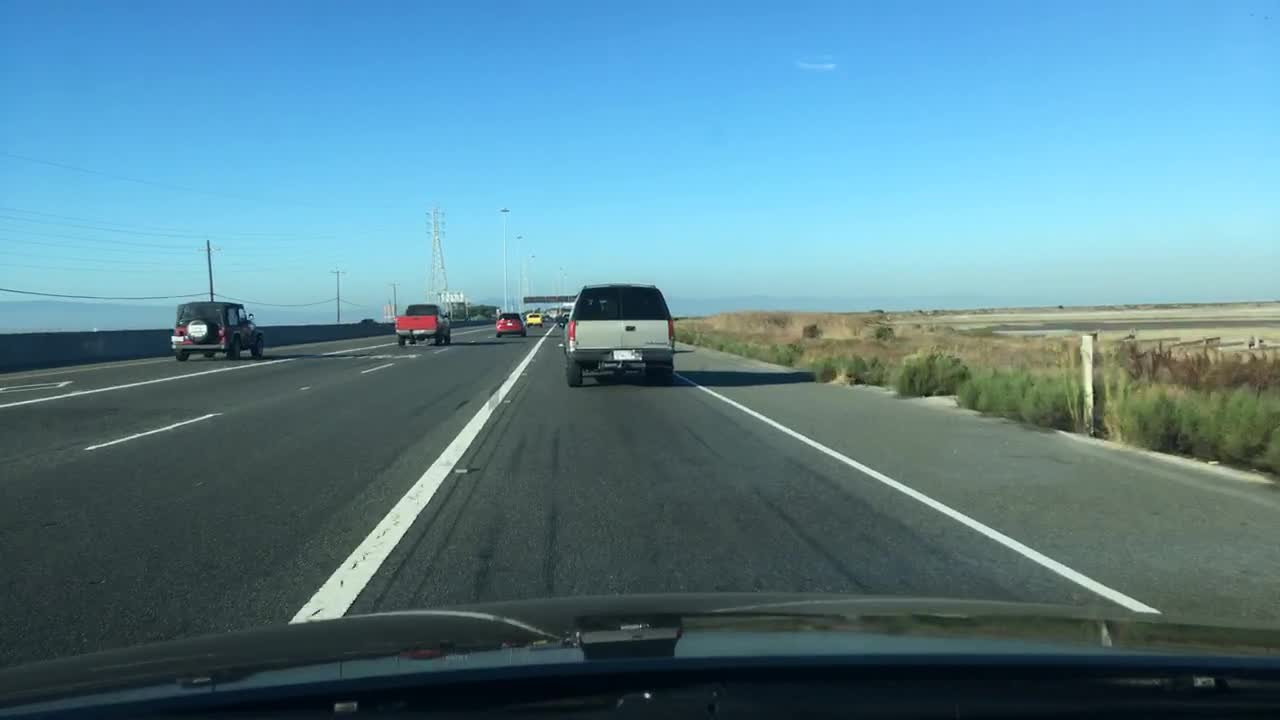
\includegraphics[width=0.4\textwidth]{0a0a0b1a-7c39d841.png} &
							
						\begin{tikzpicture}
							\draw[-to, white](0,0) -- (1,0);
							\draw[-to, thick](0,1.65) -- (1,1.65);
						\end{tikzpicture} &
							
						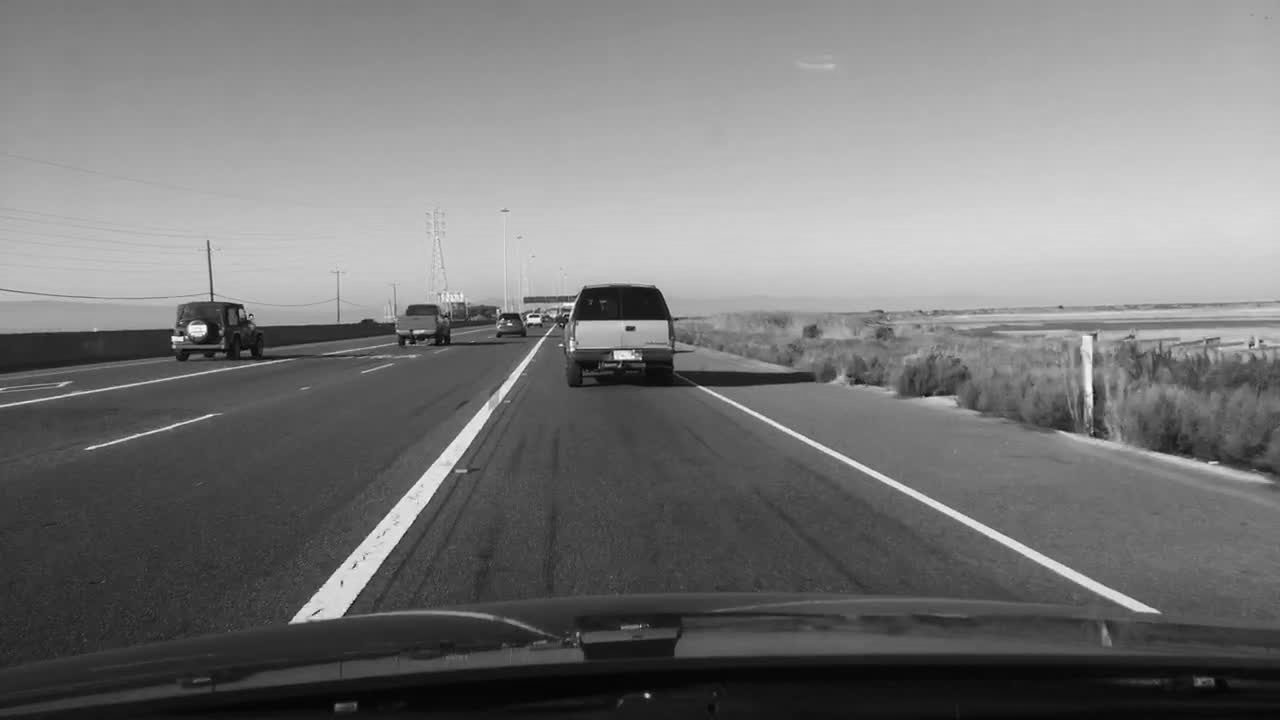
\includegraphics[width=0.4\textwidth]{0a0a0b1a-7c39d841.grayscale.out.png} \\

					\end{tabular}

				\end{figuur}

				\bigskip

				Next, I coded a function to apply a Gaussian blur to an image.
				This function takes arbitrary arguments for the standard \mbox{deviation $\sigma$ and} for the \mbox{kernel size $K_s = K_x = K_y$}.
				Note \mbox{that $K_{s} \geq 1 \wedge K_{s} \equiv 1 \bmod 2$ to be a valid size.}
				First, the function calculates the kernel values according to the mentioned parameters.
				It does this by using a derivation of the formula seen in \verwijzingb{figuur}{Formula for generating a two-dimensional Gaussian kernel} that gives the value for one value in the kernel.
				I have shown this derivation in \verwijzingb{figuur}{Formula for the weight of one value within a Gaussian kernel}, where $K_r = \frac{(K_s - 1)}{2}$ and $x,y$ are the absolute coordinates of the point within the kernel.

				\begin{figuur}{Formula for the weight of one value within a Gaussian kernel}
					
					\begin{largequation}
						K = e^{-(\frac{(y - K_r)^2 + (x - K_r)^2}{2 * \sigma^2})}
					\end{largequation}

				\end{figuur}

				\begin{figuur}{A test image blurred by a Gaussian function}

					\begin{tabular}{ccc}
								
						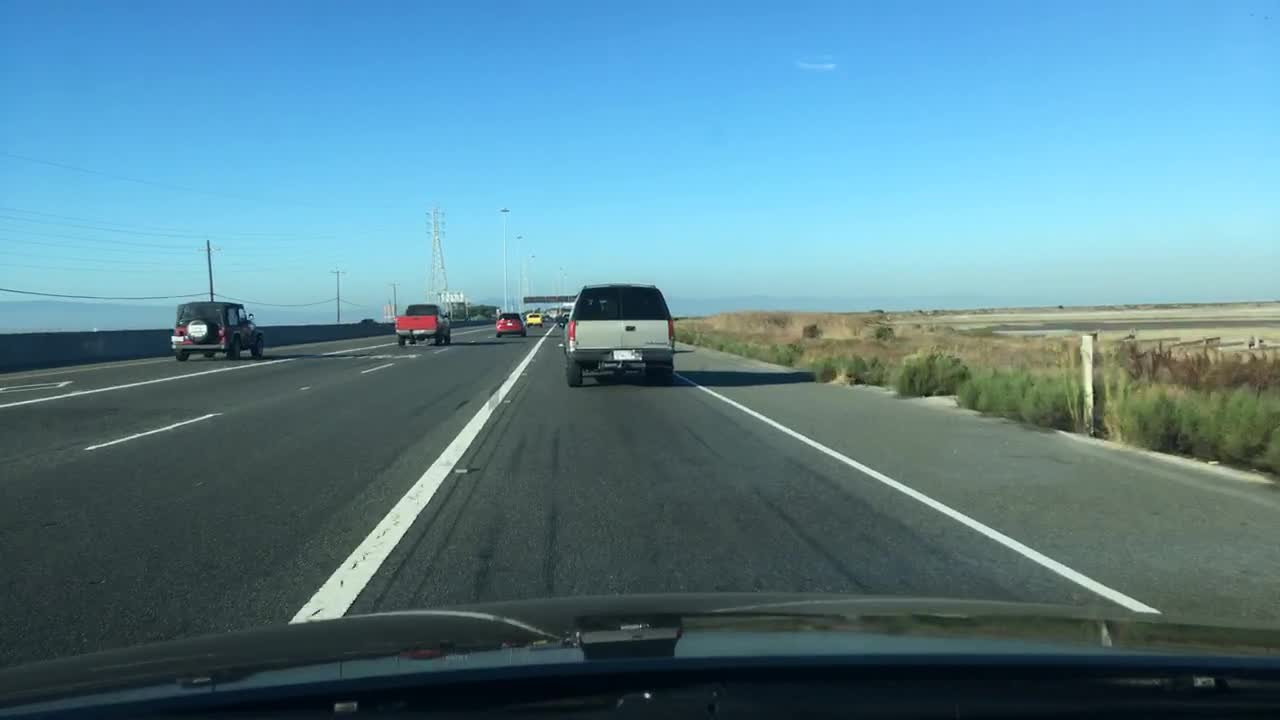
\includegraphics[width=0.4\textwidth]{0a0a0b1a-7c39d841.png} &
								
						\begin{tikzpicture}
							\draw[-to, white](0,0) -- (1,0);
							\draw[-to, thick](0,1.65) -- (1,1.65);
						\end{tikzpicture} &
						
						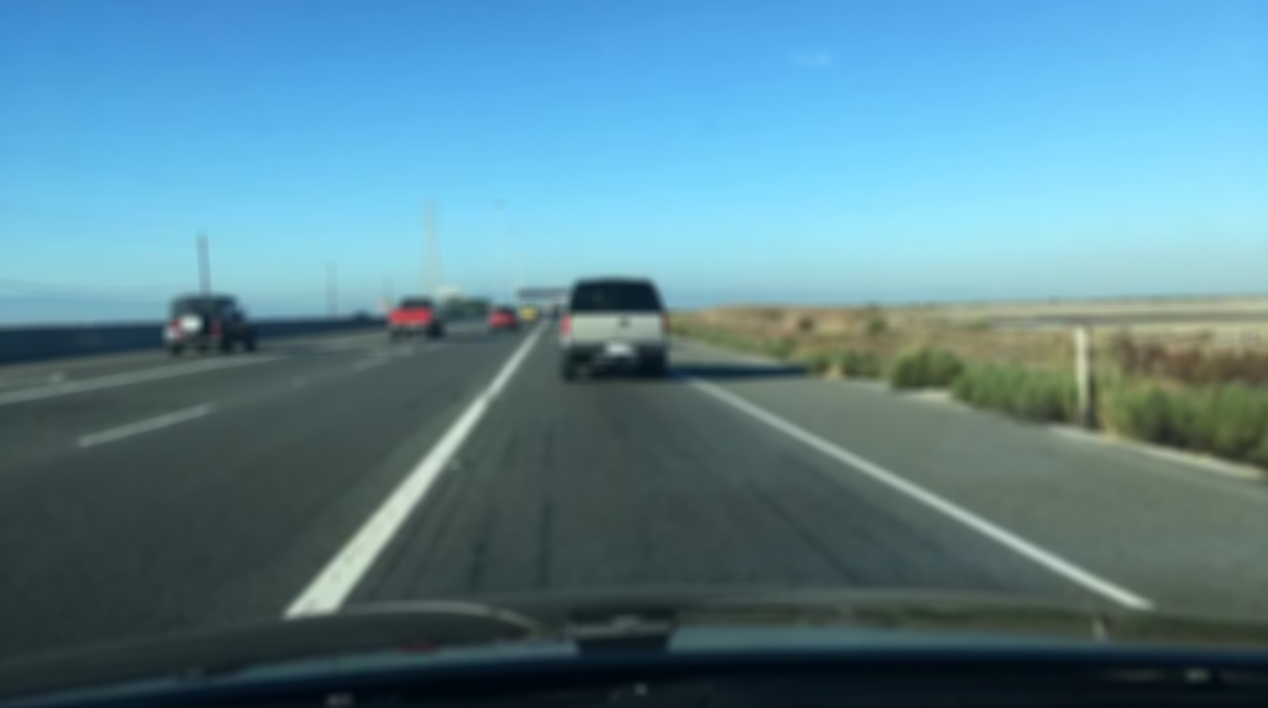
\includegraphics[width=0.4\textwidth]{0a0a0b1a-7c39d841.gaussian.out.png} \\

						&& $ K_x = K_y = 10 $ \\
						&& $ \sigma = 6,0 $
						
					\end{tabular}

				\end{figuur}

				\begin{figuur}{A grayscale test image subjected to the Sobel-Feldman operator}

					\begin{tabular}{ccc}
						
						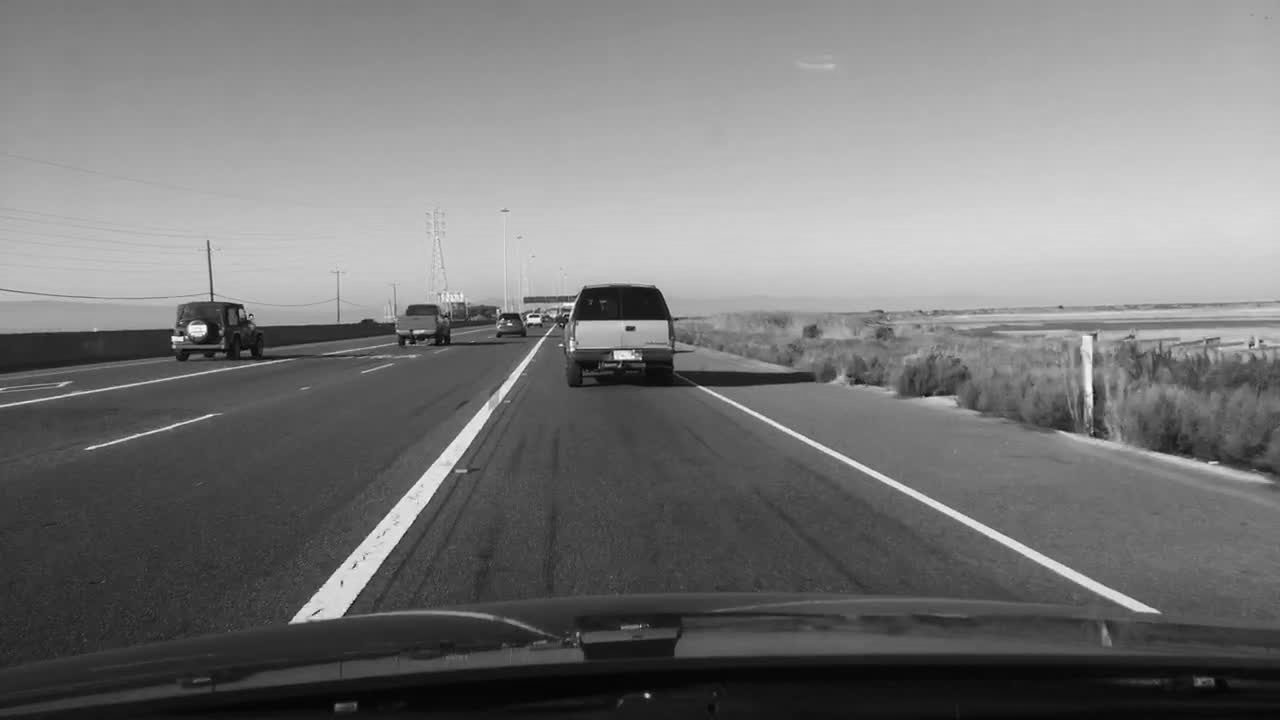
\includegraphics[width=0.4\textwidth]{0a0a0b1a-7c39d841.grayscale.out.png} &
						
						\begin{tikzpicture}
							\draw[-to, white](0,0) -- (1,0);
							\draw[-to, thick](0,1.65) -- (1,1.65);
						\end{tikzpicture} &
						
						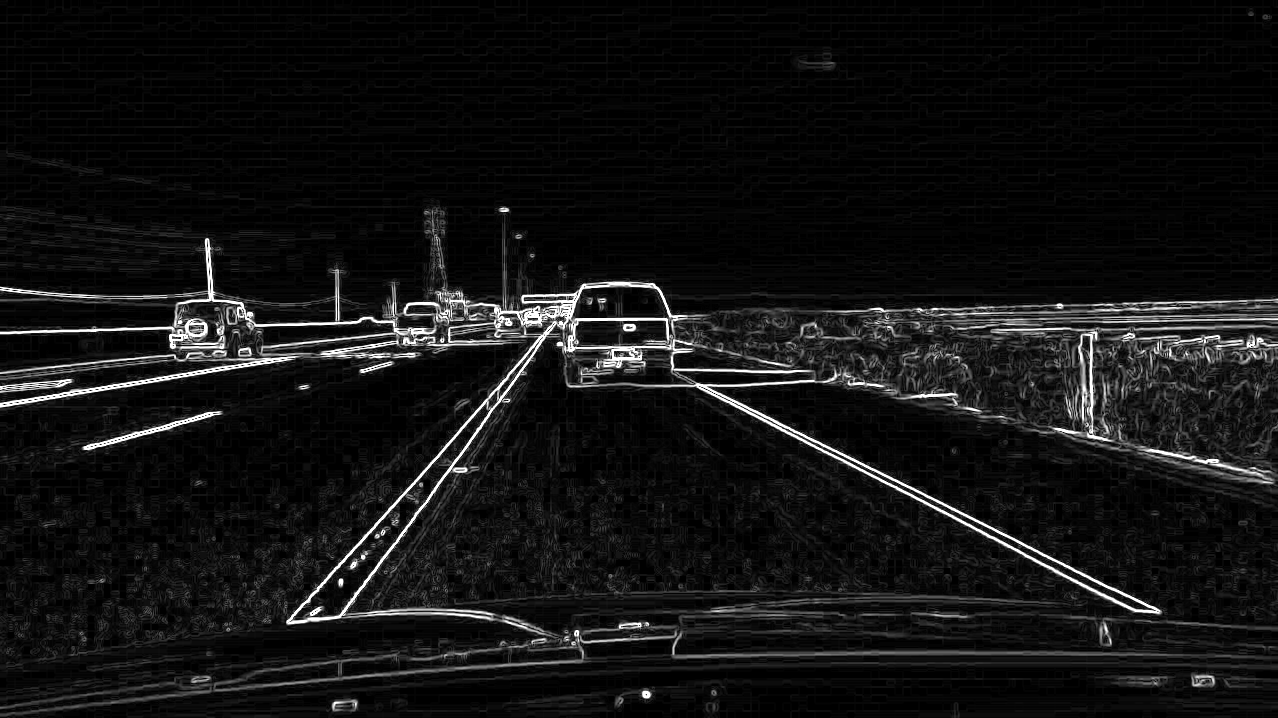
\includegraphics[width=0.4\textwidth]{0a0a0b1a-7c39d841.sobel.gn.tn.out.png}

					\end{tabular}

				\end{figuur}
			
				As can be seen in \verwijzingb{figuur}{A grayscale test image subjected to the Sobel-Feldman operator}, when we apply the Sobel operator to an unfiltered grayscale version of our test image, many photographic artifacts can be observed.
				To reduce these artifacts, it is common practice to apply noise reduction \textbf{before} applying the Sobel filter.
				An example of this, using a Gaussian blur with $ K_x=K_y=5 $ and $ \sigma = 2.1 $ beforehand, can be seen \mbox{in \verwijzingb{figuur}{A fully preprocessed test image subjected to the Sobel-Feldman operator}.}
				The difference is noticeable and because of this, although the filter is computationally expensive, I have chosen to implement the blur.

				\begin{figuur}{A fully preprocessed test image subjected to the Sobel-Feldman operator}

					\begin{tabular}{ccc}
						
						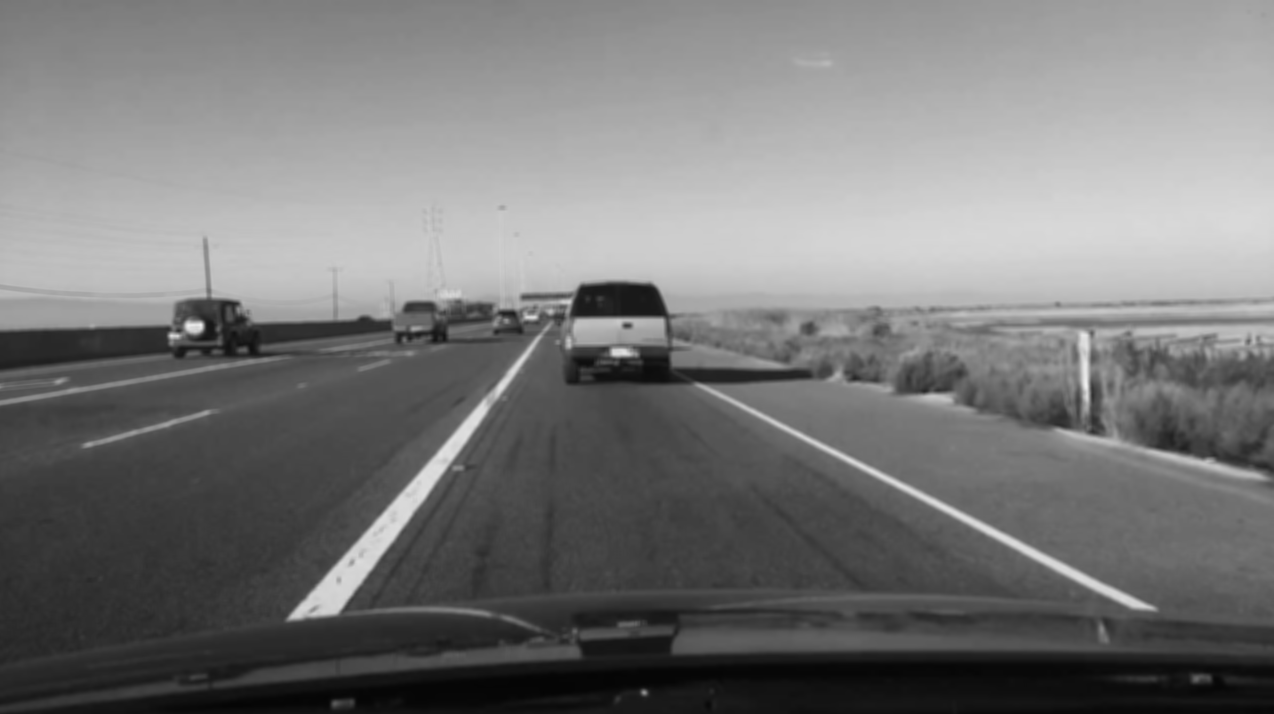
\includegraphics[width=0.4\textwidth]{0a0a0b1a-7c39d841.pre.out.png} &
						
						\begin{tikzpicture}
							\draw[-to, white](0,0) -- (1,0);
							\draw[-to, thick](0,1.65) -- (1,1.65);
						\end{tikzpicture} &
						
						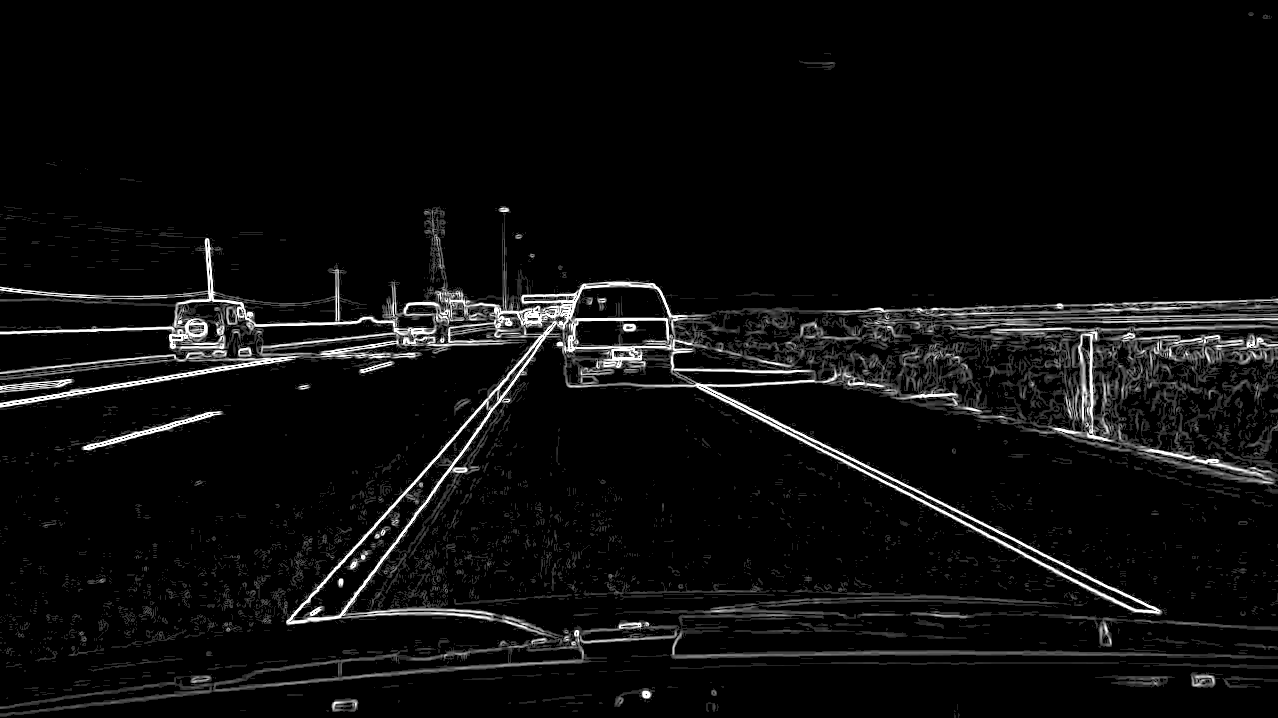
\includegraphics[width=0.4\textwidth]{0a0a0b1a-7c39d841.sobel.tn.out.png} \\
						$ K_x = K_y = 5 $ && \\
						$ \sigma = 2.1 $ \\

					\end{tabular}

				\end{figuur}

				If we apply a threshold with an intensity of $ T_G = 80\% $ to the output of the Sobel operator seen \mbox{in \verwijzingb{figuur}{A fully preprocessed test image subjected to the Sobel-Feldman operator} we} can discard a lot of artifacts from the image.
				The result of this operation can be seen \mbox{in \verwijzingb{figuur}{Example of thresholding applied to the output of the Sobel-Feldman operator}.}
				The lane markings persist, but many of the details in the roadside get discarded.

				\begin{figuur}{Example of thresholding applied to the output of the Sobel-Feldman operator}

					\begin{tabular}{ccc}
							
						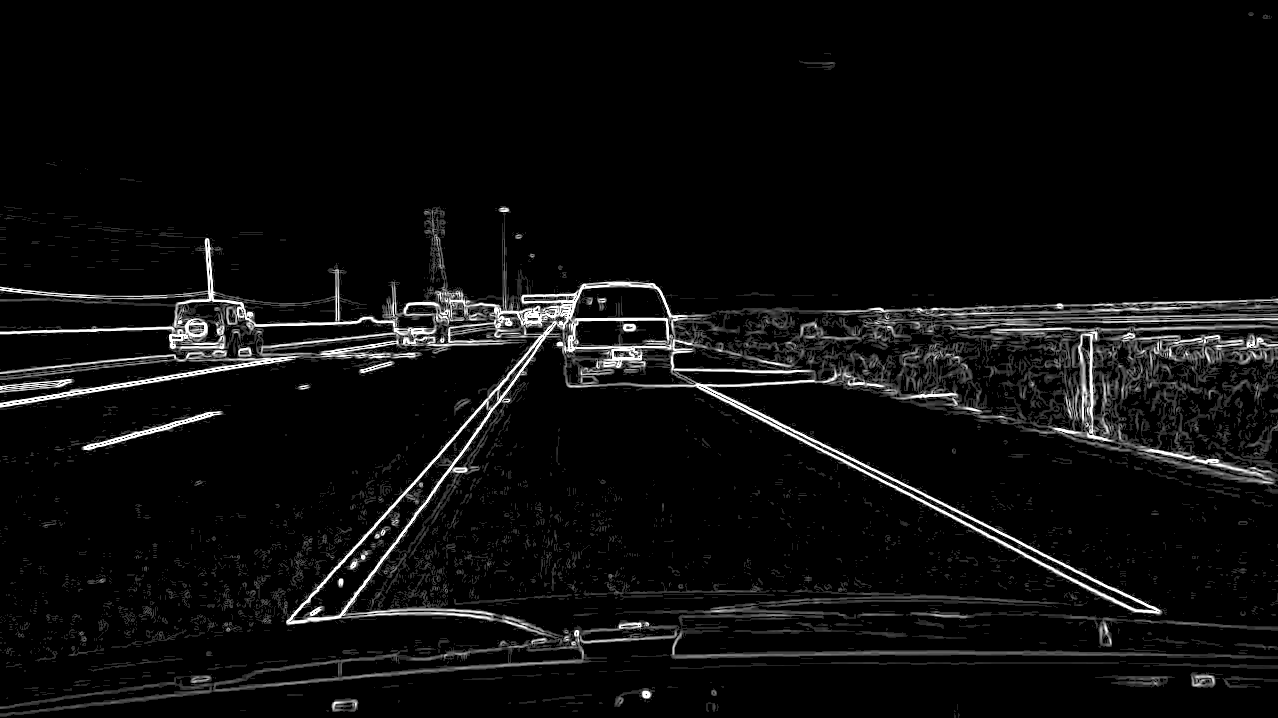
\includegraphics[width=0.4\textwidth]{0a0a0b1a-7c39d841.sobel.tn.out.png} &
							
						\begin{tikzpicture}
							\draw[-to, white](0,0) -- (1,0);
							\draw[-to, thick](0,1.65) -- (1,1.65);
						\end{tikzpicture} &
							
						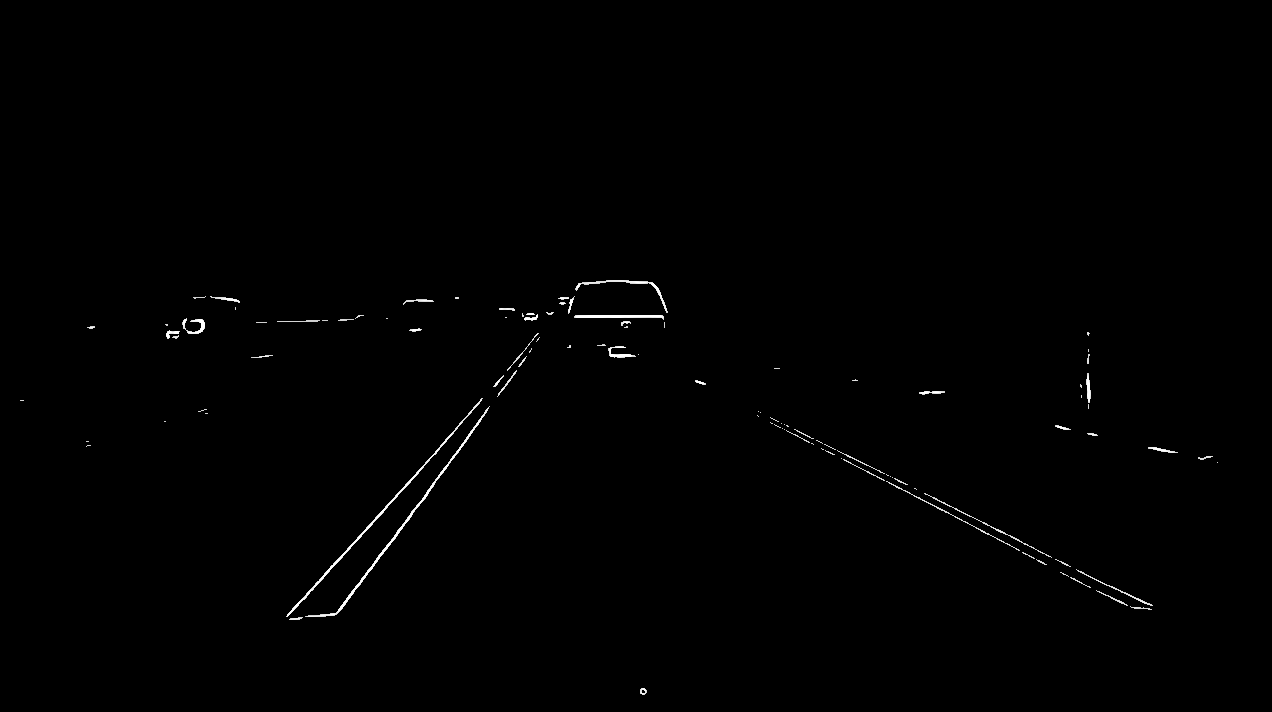
\includegraphics[width=0.4\textwidth]{0a0a0b1a-7c39d841.sobel.out.png} \\

						&& $ T_G = 80\% $
					\end{tabular}

				\end{figuur}

			\end{subparagraaf}

			\begin{subparagraaf}{Hough Transform Implementation}
		
				The range of orientations of the Hough Transform can be fitted in two ways: $\pi \leq \theta < 0$ where $\rho$ holds both negative and positive values, or $0 \leq \theta < \pi$ where $\rho$ holds only positive values \cite{anvari2010fpga}.
				I chose to go with the former approach because it allows the use of fixed point values, which is useful when implementing it in digital logic.
				This is the reason why in my implementation, the height of the Hough space is $\sqrt{2} \cdot I_x$ where $I_x$ is the image width.
				I also considered the Hough-Green transform as proposed by Shapiro et al. \cite{shapiro2006accuracy} because it is a kernel-based approach, but I realized that it would require even more memory operations than the classical Hough transform due to it needing information about neighbor pixels during the voting phase.

				\begin{figuur}{A test image processed with Hough Transform using a too low threshold}

					\begin{tabular}{ccc}
							
						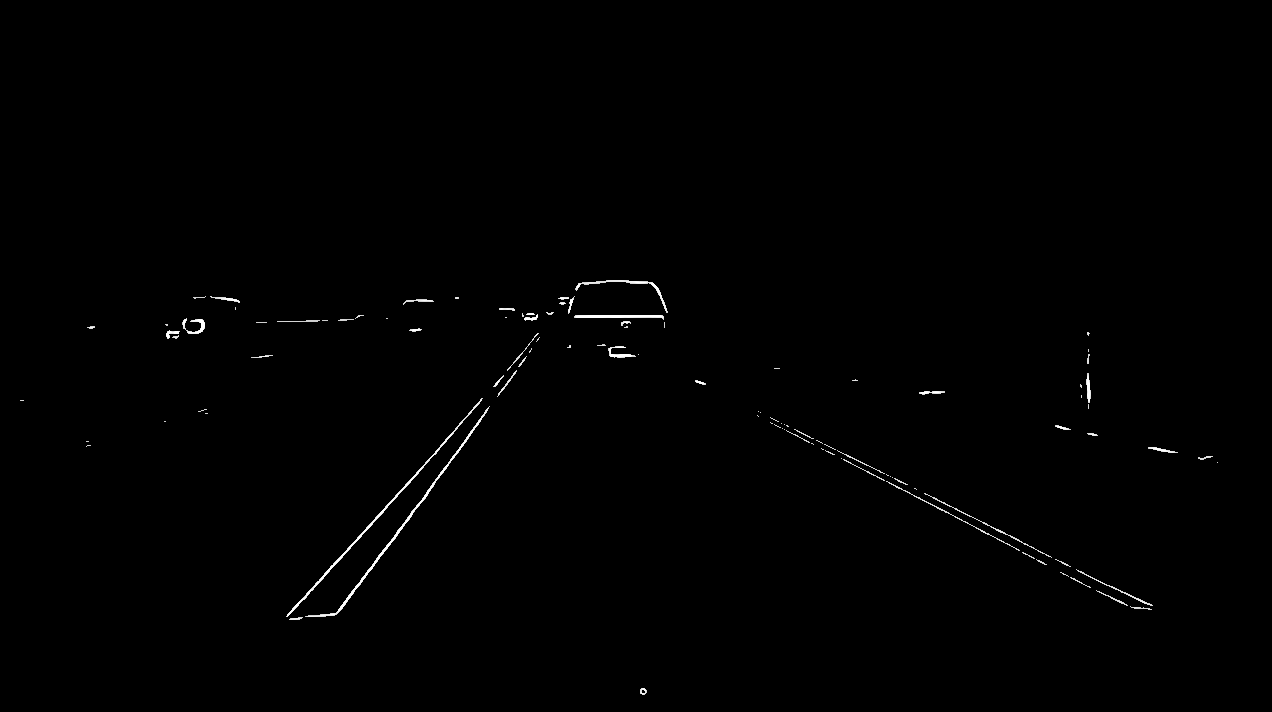
\includegraphics[width=0.4\textwidth]{0a0a0b1a-7c39d841.sobel.out.png} &
							
						\begin{tikzpicture}
							\draw[-to, white](0,0) -- (1,0);
							\draw[-to, thick](0,1.65) -- (1,1.65);
						\end{tikzpicture} &
							
						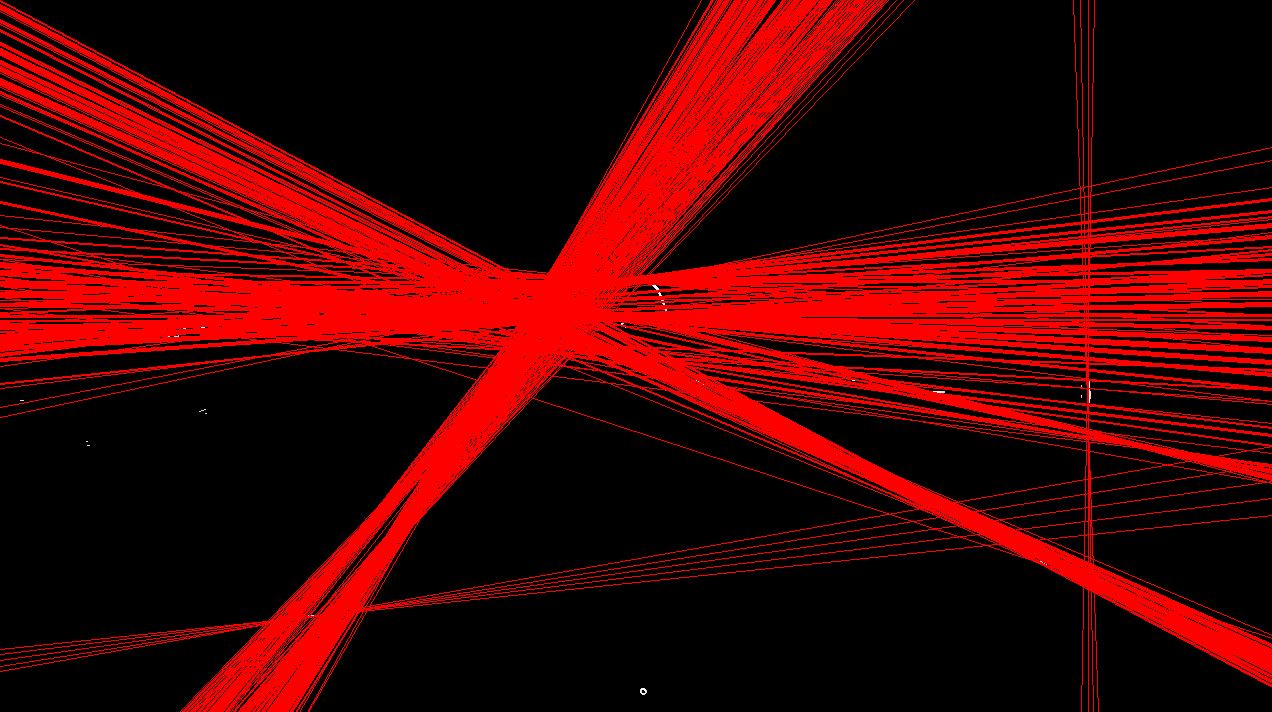
\includegraphics[width=0.4\textwidth]{0a0a0b1a-7c39d841.hough-t40.out.png} \\

														       && $ T_H \approx 15\% $
					\end{tabular}

				\end{figuur}

				\bigskip

				The threshold of the peaks in the histogram can be arbitrarily modified in my Hough implementation.
				I first tested the implementation on the output of \verwijzingb{figuur}{Example of thresholding applied to the output of the Sobel-Feldman operator} with $ T_H \approx 15\% $, which resulted in \verwijzingb{figuur}{A test image processed with Hough Transform using a too low threshold}.
				As can be seen in the image, many lines get picked up including roadside artifacts and those from the outline of the car in front.
			
				\begin{figuur}{A test image processed with Hough Transform using a reasonable threshold}

					\begin{tabular}{ccc}
							
						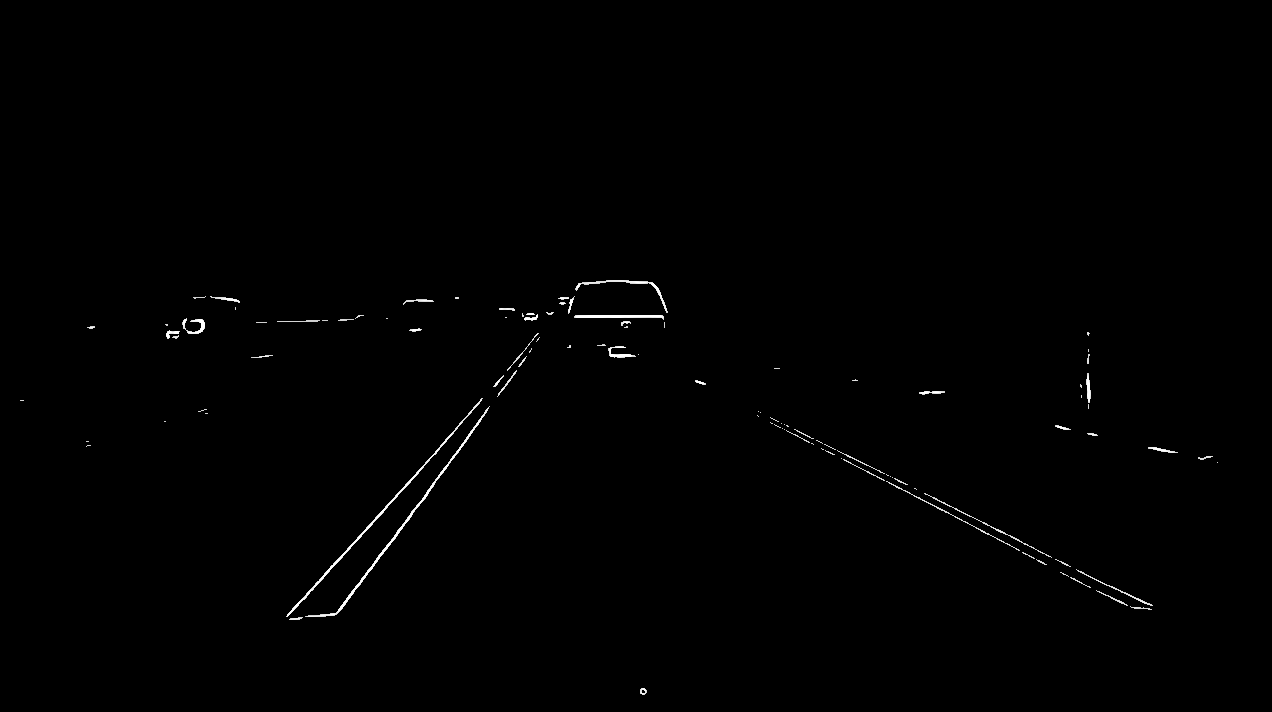
\includegraphics[width=0.4\textwidth]{0a0a0b1a-7c39d841.sobel.out.png} &
							
						\begin{tikzpicture}
							\draw[-to, white](0,0) -- (1,0);
							\draw[-to, thick](0,1.65) -- (1,1.65);
						\end{tikzpicture} &
							
						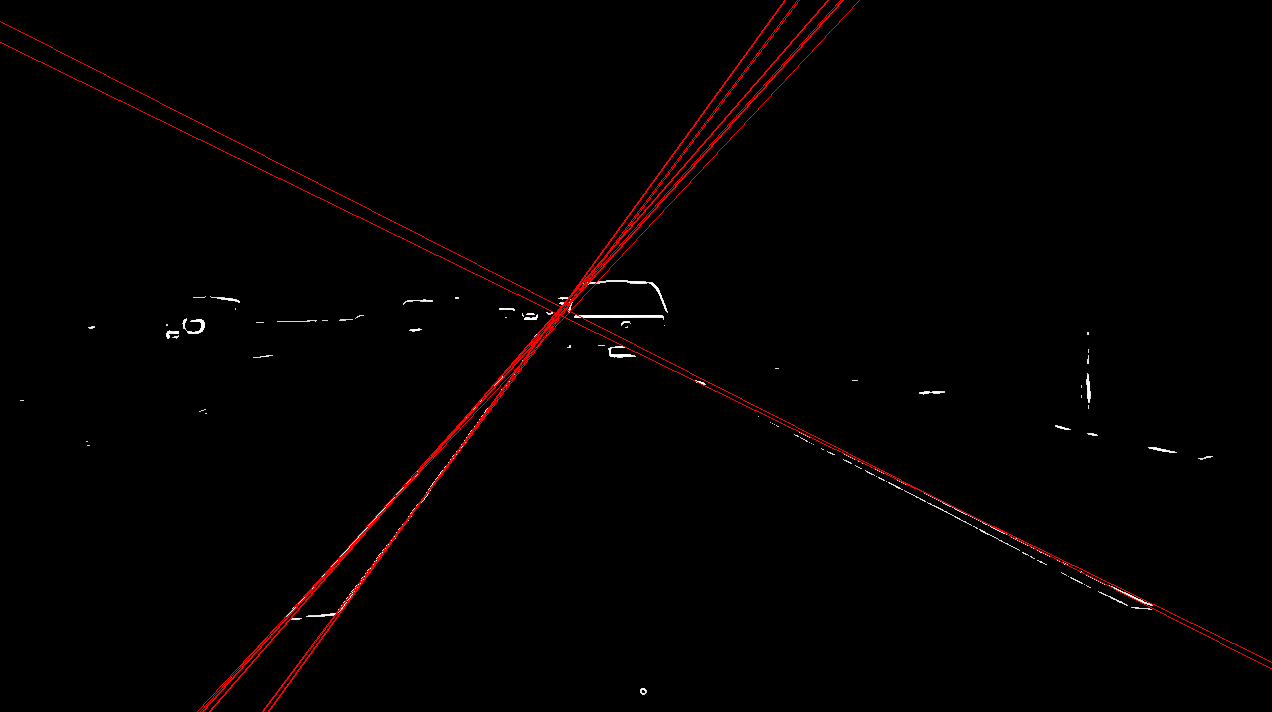
\includegraphics[width=0.4\textwidth]{0a0a0b1a-7c39d841.hough-t150.out.png} \\

						&& $ T_H \approx 60\% $ 
					\end{tabular}

				\end{figuur}

				\bigskip

				After some testing, I found that thresholds around 60 percent worked well with the images from the test dataset.
				Though, for the end product to be suitable for many different environments, this threshold needs to be configurable.
				Using the value of 60 percent on the output of \verwijzingb{figuur}{Example of thresholding applied to the output of the Sobel-Feldman operator} resulted in \verwijzingb{figuur}{A test image processed with Hough Transform using a reasonable threshold}.
				The Hough space that resulted from this transformation is visualized in \verwijzingb{figuur}{Hough space visualization of Figure \getrefnumber{figuur:A test image processed with Hough Transform using a reasonable threshold} as a graph}.
				In this figure, the luminance of each pixel is the raw accumulator value, capped at the value of 255 because of color channel size restrictions.
				The white blobs near $(50,400)$ represent the left lane marking.
				The two clearly defined peaks near $(150,500)$ represent the edges of the right lane marking.
				If we overlay a polar grid as in \verwijzingb{figuur}{Polar grid overlay applied to Figure \getrefnumber{figuur:A test image processed with Hough Transform using a reasonable threshold} centered on the vanishing point}, we can see that the $\theta$-values match up.
				This proves that my implementation of the Hough Transform is correct.

				\begin{figuur}{Hough space visualization of Figure \getrefnumber{figuur:A test image processed with Hough Transform using a reasonable threshold} as a graph}

					% ok dit is echt hele lelijke code...
					\begin{tikzpicture}
					
						\node[anchor=south west, inner sep=0] (image) at (0,0) {
							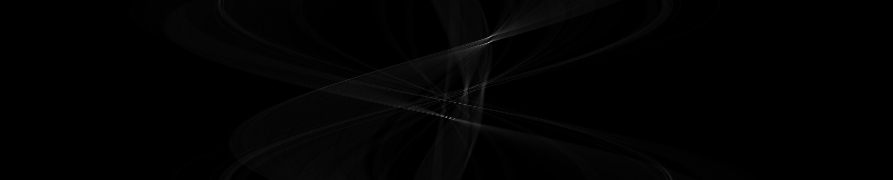
\includegraphics[width=0.8\textwidth]{0a0a0b1a-7c39d841.hough-t150-histogram.out.png}
						};

						\begin{scope}[x={(image.south east)}, y={(image.north west)}]
							
%							\draw[help lines, xstep=.1, ystep=.25] (0,0) grid (1,1);

							% horizontale lijnen
							\draw [black, anchor=north] (0,-0.05) to (1,-0.05);
							\foreach \x in {0,1,...,5} {
								\node [anchor=north] at (\x*2/10,-0.13) {{\footnotesize\the\numexpr\x*180\relax}};
								\draw [black, anchor=north] (\x/5,-0.05) to (\x/5,-0.13);
							}
							\foreach \x in {0,1,...,20} {
								\draw [black, anchor=north] (\x/20,-0.05) to (\x/20,-0.10);
							}
%							\node[anchor=north] at (0.1,-0.13) {{\footnotesize$\rho$}};
							
							\node[anchor=north east] at (-0.0195, -0.13) {{$(\small\theta,\rho)$}};

							% verticale lijnen
							\draw [black] (-0.0095,0) to (-0.0095,1);
							\foreach \y in {0,1,...,4} {
								\node [anchor=east] at (-0.0295,\y*2.5/10) {{\footnotesize\the\numexpr\y*45\relax}};
								\draw [black, anchor=east] (-0.0095,\y*2.5/10) to (-0.0295,\y*2.5/10);

							}
							
						\end{scope}

					\end{tikzpicture}

				\end{figuur}

				\begin{figuur}{Polar grid overlay applied to Figure \getrefnumber{figuur:A test image processed with Hough Transform using a reasonable threshold} centered on the vanishing point}

					\begin{tikzpicture}

						\begin{polaraxis}[
							grid=both,
							xmin=0,xmax=180,
							ytick=\empty,
							minor tick num=5
							]

							\addplot[white,color=white] coordinates {(1,1)};
							\node[] at (rel axis cs:0,0) {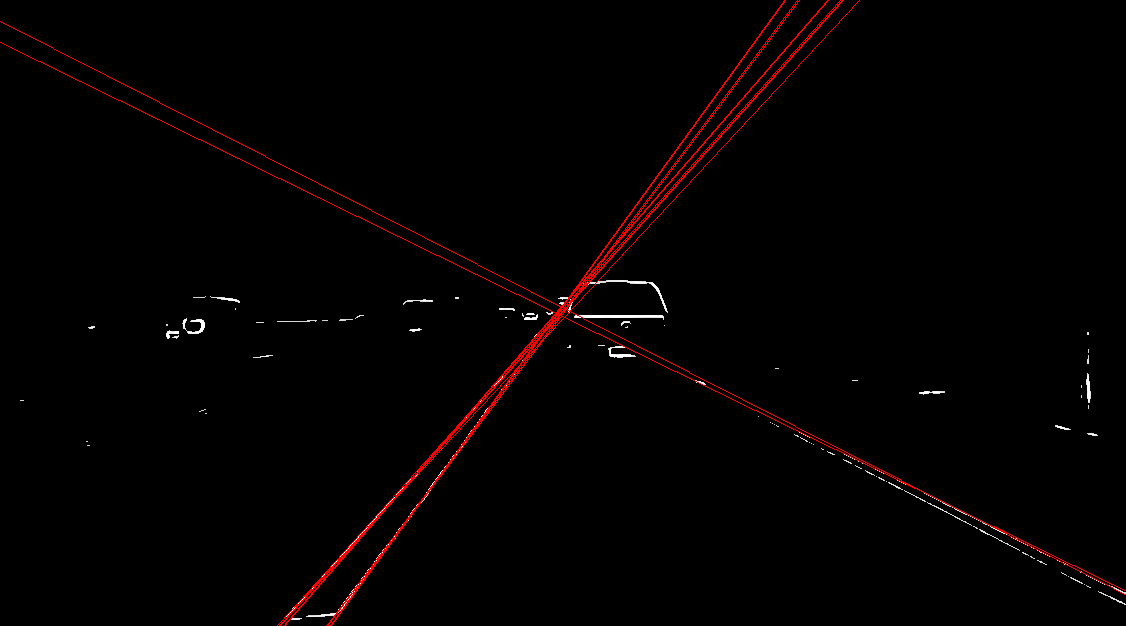
\includegraphics[width=0.9\textwidth]{0a0a0b1a-7c39d841.hough-t150.out.crop.png}};

						\end{polaraxis}
					\end{tikzpicture}

				\end{figuur}

			\end{subparagraaf}

			\begin{subparagraaf}{$k$-means Implementation}

				As can be seen in \verwijzingb{figuur}{Hough space visualization of Figure \getrefnumber{figuur:A test image processed with Hough Transform using a reasonable threshold} as a graph}, multiple lines are left over per lane marking.
				To get the average of these results, I decided to implement Lloyd's algorithm.
				Because we don't determine the exact start and end of the detected lines, we can't use an approach like Ebrahimpour et al. \cite{ebrahimpour2012vanishing} did.
				Therefore, I decided to cluster the lines based on their angle.
				I figured that the lines from the left lane marking will always have $\theta < 90$ and those from the right marking will have $\theta > 90$.
				Lloyd's algorithm is suited for multidimensional datasets, but I decided to try it in a one-dimensional way and see if it works.

			\end{subparagraaf}

		\end{paragraaf}

		\begin{paragraaf}{The Final Chosen Pipeline}

			After having researched the widely used candidate algorithms and having implemented them myself, I am able to judge which of these algorithms would make up a sufficient lane detection pipeline.
			I decide to implement a pipeline using the following algorithms sequentially:

			\begin{enumerate}

				\item	Grayscale conversion -- this strategy is widely used to turn the input video frame from the camera into a single-channel image composed only of the luminance of each pixel.
					The advantages of using grayscale images is that less memory is required to store them and less computational power is required to process them, while keeping the same information.
				\item	Gaussian blur -- from the testing done using the sample data, it turns out that lots of noise gets eliminated from the picture if the image is blurred before the edge detection operator is applied.
					Therefore, I decided that it is worthwile to implement a Gaussian filter.
				\item	Sobel operator -- I decided to use the plain Sobel operator instead of the full-fledged Canny Edge Detector because the latter didn't provide a much better result to make it worth my time.
					The plain Sobel operator clearly defines the edges in every sample picture while being relatively simple to implement.
				\item	Thresholding -- The output from the Sobel operator is still measured in a luminance values, meaning we have to convert it to a binary image first by applying a threshold.
					This technique is easy to implement and my testing concluded that it reduces a lot of the leftover image artifacts.
				\item	Hough Transform -- Although it is challenging to implement this algorithm on an FPGA, numerous research papers have suggested different ways of implementing it, making it well documented.
					Because there are multiple approaches to implementing it on a FPGA, I think it will be possible for me to achieve this.
					I chose the Hough Transform over other methods because it is perfect for detecting dashed lines, which makes it perfect for detecting lane markings.
				\item	$k$-means clustering -- To group the results from the Hough Transform, I decided to use a clustering technique.
					I chose to use $k$-means clustering over DBSCAN because the former only requires one parameter -- the cluster size -- which we know beforehand.
					The parameters used in DBSCAN clustering depend on a given situation and need to be configured afterwards, making it harder to implement.

			\end{enumerate}

		\end{paragraaf}

	\end{hoofdstuk}

	\begin{hoofdstuk}{Conclusion}

		\textbf{[todo:]}

	\end{hoofdstuk}

	\begin{hoofdstuk}{Discussion}

		\textbf{[todo:]}

	\end{hoofdstuk}

	% Bibliography page
	\begin{hoofdstuk}{References}

		\printbibliography[heading=none]
	
	\end{hoofdstuk}

	% Empty last page
	\clearpage
	\thispagestyle{empty}
	\addtocounter{page}{-1}
	\ThisULCornerWallPaper{1.005}{asset_bg_last_page.jpg}
	\
	\clearpage

\end{document}
